% A LaTeX template for EXECUTIVE SUMMARY of the MSc Thesis submissions to
% Politecnico di Milano (PoliMi) - School of Industrial and Information Engineering
%
% P. F. Antonietti, S. Bonetti, A. Gruttadauria, G. Mescolini, A. Zingaro
% e-mail: template-tesi-ingind@polimi.it
%
% Last Revision: October 2021
%
% Copyright 2021 Politecnico di Milano, Italy. Inc. All rights reserved.

\documentclass[12pt,a4paper]{article}

%------------------------------------------------------------------------------
%	REQUIRED PACKAGES AND  CONFIGURATIONS
%------------------------------------------------------------------------------
% PACKAGES FOR TITLES
\usepackage{titlesec}
\usepackage{color}

% PACKAGES FOR LANGUAGE AND FONT
\usepackage[utf8]{inputenc}
\usepackage[english]{babel}
\usepackage[T1]{fontenc} % Font encoding
\usepackage{comment}

% PACKAGES FOR IMAGES
\usepackage{graphicx}
\graphicspath{{imgs/}} % Path for images' folder
\usepackage{eso-pic} % For the background picture on the title page
%\usepackage{subfig} % Numbered and caption subfigures using \subfloat
\usepackage{subcaption}
\usepackage[font=small]{caption} % Coloured captions
\usepackage{transparent}

% STANDARD MATH PACKAGES
\usepackage{amsmath}
\usepackage{amsthm}
\usepackage{amsfonts}    % added for project
\usepackage{bm}
\usepackage[overload]{empheq}  % For braced-style systems of equations

% PACKAGES FOR TABLES
\usepackage{tabularx}
\usepackage{longtable} % tables that can span several pages
\usepackage{colortbl}

% PACKAGES FOR ALGORITHMS (PSEUDO-CODE)
\usepackage{algorithm}
\usepackage{algorithmic}

% PACKAGES FOR REFERENCES & BIBLIOGRAPHY
\usepackage[colorlinks=true,linkcolor=black,anchorcolor=black,citecolor=black,filecolor=black,menucolor=black,runcolor=black,urlcolor=black]{hyperref} % Adds clickable links at references
\usepackage{cleveref}
% \usepackage[square, numbers, sort&compress]{natbib} % Square brackets, citing references with numbers, citations sorted by appearance in the text and compressed
\usepackage[
    backend=biber,
    style=alphabetic,
]{biblatex}
\addbibresource{bibliography.bib} 
\usepackage{csquotes}
% \bibliographystyle{apalike} % You may use a different style adapted to your field

% PACKAGES FOR THE APPENDIX
\usepackage{appendix}

% PACKAGES FOR ITEMIZE & ENUMERATES
\usepackage{enumitem}

% OTHER PACKAGES
\usepackage{amsthm,thmtools,xcolor} % Coloured "Theorem"
\usepackage{comment} % Comment part of code
\usepackage{fancyhdr} % Fancy headers and footers
\usepackage{lipsum} % Insert dummy text
\usepackage{tcolorbox} % Create coloured boxes (e.g. the one for the key-words)
\usepackage{stfloats} % Correct position of the tables

%-------------------------------------------------------------------------
%	NEW COMMANDS DEFINED
%-------------------------------------------------------------------------
% EXAMPLES OF NEW COMMANDS -> here you see how to define new commands
\newcommand{\bea}{\begin{eqnarray}} % Shortcut for equation arrays
\newcommand{\eea}{\end{eqnarray}}
\newcommand{\e}[1]{\times 10^{#1}}  % Powers of 10 notation
\newcommand{\mathbbm}[1]{\text{\usefont{U}{bbm}{m}{n}#1}} % From mathbbm.sty
\newcommand{\pdev}[2]{\frac{\partial#1}{\partial#2}}

\newcommand{\ppmSuite}{\texttt{ppmSuite}}
\newcommand{\drpm}{\texttt{drpm}}

\DeclareMathOperator{\Normal}{\mathcal{N}}
\DeclareMathOperator{\DD}{\mathcal{D}}
\DeclareMathOperator{\indicator}{\pmb{1}}
\DeclareMathOperator{\tRPM}{\mathrm{tRPM}}
\DeclareMathOperator{\PPMx}{\mathrm{PPMx}}
\DeclareMathOperator{\sPPM}{\mathrm{sPPM}}
\DeclareMathOperator{\NormInvWish}{\mathrm{NIW}}
\DeclareMathOperator{\Uniform}{\mathrm{UN}}
\DeclareMathOperator{\BetaDist}{\mathrm{Beta}}
\DeclareMathOperator{\Bernoulli}{\mathrm{Ber}}
\DeclareMathOperator{\RR}{\mathbb{R}}
\DeclareMathOperator{\Identity}{\mathrm{Id}}
\DeclareMathOperator{\PosSemDef}{\mathbb{S}}
\DeclareMathOperator{\PP}{\mathbb{P}}
\DeclareMathOperator{\Multinomial}{\mathrm{Multinomial}}
\DeclareMathOperator{\Laplace}{\mathrm{Laplace}}
\DeclareMathOperator{\Dir}{\mathrm{Dirichlet}}
\newcommand*{\tran}{^{\mkern-1.5mu\mathsf{T}}}
\newcommand*{\ind}{\overset{\tiny{\textrm{ind}}}{\sim}}
\newcommand*{\iid}{\overset{\tiny{\textrm{iid}}}{\sim}}

%----------------------------------------------------------------------------
%	ADD YOUR PACKAGES (be careful of package interaction)
%----------------------------------------------------------------------------

\usepackage{physics}
\usepackage{amssymb}
\usepackage{aligned-overset}
% for correct scientific tables
\usepackage{tabularx}
\usepackage{booktabs}
% for subfigures
\usepackage{subcaption}
\usepackage{graphicx}
\usepackage{caption}


%----------------------------------------------------------------------------
%	ADD YOUR DEFINITIONS AND COMMANDS (be careful of existing commands)
%----------------------------------------------------------------------------


% Do not change Configuration_files/config.tex file unless you really know what you are doing.
% This file ends the configuration procedures (e.g. customizing commands, definition of new commands)
% Set the geometric layout of the document
\usepackage{geometry}
\geometry{
  top=3cm,
  left = 2.0cm,
  right = 2.75cm,
  bottom=2cm,
  headheight= 2cm,
  headsep= 0cm,
}
\raggedbottom 

% Create color bluePoli (-> manuale grafica coordinata:  https://www.polimi.it/fileadmin/user_upload/il_Politecnico/grafica-coordinata/2015_05_11_46xy_manuale_grafica_coordinata.pdf)
\definecolor{bluePoli}{cmyk}{0.4,0.1,0,0.4}

% Custom theorem environments
\declaretheoremstyle[
  headfont=\color{bluePoli}\normalfont\bfseries,
  bodyfont=\color{black}\normalfont\itshape,
]{colored}

\captionsetup[figure]{labelfont={color=bluePoli}} % Set colour of the captions
\captionsetup[table]{labelfont={color=bluePoli}} % Set colour of the captions
\captionsetup[algorithm]{labelfont={color=bluePoli}} % Set colour of the captions

\theoremstyle{colored}
\newtheorem{theorem}{Theorem}[section]
\newtheorem{proposition}{Proposition}[section]

% Enhances the features of the standard "table" and "tabular" environments.
\newcommand\T{\rule{0pt}{2.6ex}}
\newcommand\B{\rule[-1.2ex]{0pt}{0pt}}

% Algorithm description
\newcounter{algsubstate}
\renewcommand{\thealgsubstate}{\alph{algsubstate}}
\newenvironment{algsubstates}{
    \setcounter{algsubstate}{0}%
    \renewcommand{\STATE}{%
    \stepcounter{algsubstate}%
    \Statex {\small\thealgsubstate:}\space}
    }{}
    
% Custom theorem environment
\newcolumntype{L}[1]{>{\raggedright\let\newline\\\arraybackslash\hspace{0pt}}m{#1}}
\newcolumntype{C}[1]{>{\centering\let\newline\\\arraybackslash\hspace{0pt}}m{#1}}
\newcolumntype{R}[1]{>{\raggedleft\let\newline\\\arraybackslash\hspace{0pt}}m{#1}}

% Custom itemize environment
\setlist[itemize,1]{label=$\bullet$}
\setlist[itemize,2]{label=$\circ$}
\setlist[itemize,3]{label=$-$}
\setlist{nosep}

% Set separation of columns 
\setlength{\columnsep}{30pt}

% Create command for background pic
\newcommand\BackgroundPic{% Adding background picture
	\put(230,358){
		\parbox[b][\paperheight]{\paperwidth}{%
			\vfill
			\centering
			\transparent{0.4}
			
\includegraphics[width=0.5\paperwidth]{logo/raggiera_polimi.eps}%
			\vfill
}}}

% Set indentation
% \setlength\parindent{0pt}

% Custom title commands
\titleformat{\section}
{\color{bluePoli}\normalfont\Large\bfseries}
{\color{bluePoli}\thesection.}{1em}{}
\titlespacing*{\section}
{0pt}{2ex}{1ex}

\titleformat{\subsection}
{\color{bluePoli}\normalfont\large\bfseries}
{\color{bluePoli}\thesubsection.}{1em}{}
\titlespacing*{\subsection}
{0pt}{2ex}{1ex}

% Custom headers and footers
\pagestyle{fancy}
\fancyhf{}
      
\fancyfoot{}
\fancyfoot[C]{\thepage} % page
\renewcommand{\headrulewidth}{0mm} % headrule width
\renewcommand{\footrulewidth}{0mm} % footrule width

\makeatletter
\patchcmd{\headrule}{\hrule}{\color{black}\hrule}{}{} % headrule
\patchcmd{\footrule}{\hrule}{\color{black}\hrule}{}{} % footrule
\makeatother

% -> Create the header
\chead[C]{
\centering
\begin{tcolorbox}[arc=0pt, boxrule=0pt, colback=bluePoli!60, width=\textwidth, colupper=white]
    \textbf{} \hfill \textbf{E. Borrini, F. Carbonara, B. Cefaloni, D. Ettel,
    A. Grignani, F. Wolf} 
\end{tcolorbox}
}

% Insert here the info that will be displayed into your Title page 
% -> title of your work
\renewcommand{\title}{CLUSTERING WEEKLY DATA OF ONE YEAR OF PM2.5 DATA}
% -> author name and surname
\renewcommand{\author}{Borrini Elisa, Carbonara Filippo, Cefaloni Benedetta, Ettel Dina Sophie, Grignani Alessandro, Wolf Florian}
% -> MSc course
\newcommand{\course}{Mathematical Engineering -- Ingegneria Matematica}
% -> advisor name and surname
\newcommand{\advisor}{Prof. Alessandra Guglielmi}
% IF AND ONLY IF you need to modify the co-supervisors you also have to modify the file Configuration_files/title_page.tex (ONLY where it is marked)
%\newcommand{\firstcoadvisor}{} % insert if any otherwise comment
%\newcommand{\secondcoadvisor}{Name Surname} % insert if any otherwise comment
% -> academic year
\newcommand{\YEAR}{2023-2024}

%-------------------------------------------------------------------------
%	BEGIN OF YOUR DOCUMENT
%-------------------------------------------------------------------------
\begin{document}

%-----------------------------------------------------------------------------
% TITLE PAGE
%-----------------------------------------------------------------------------
% Do not change Configuration_files/TitlePage.tex (Modify it IF AND ONLY IF you need to add or delete the Co-advisors)
% This file creates the Title Page of the document
% DO NOT REMOVE SPACES BETWEEN LINES!

%\twocolumn[{\begin{@twocolumnfalse}

\AddToShipoutPicture*{\BackgroundPic}

\hspace{-0.6cm}
\includegraphics[width=0.6\textwidth]{logo/logo_polimi_ing_indinf.eps}

\vspace{-1mm}
\fontsize{0.3cm}{0.5cm}\selectfont \bfseries \textsc{\color{bluePoli} Bayesian Statistics Project Final Report}\\

\vspace{-0.2cm}
\Large{\textbf{\color{bluePoli}{\title}}}\\

\vspace{-0.2cm}
\fontsize{0.3cm}{0.5cm}\selectfont \bfseries \textsc{\color{bluePoli} Laurea Magistrale in Mathematical Engineering}\\

\vspace{-0.2cm}
\fontsize{0.3cm}{0.5cm} \selectfont \bfseries Authors: \textsc{\textbf{\author}}\\

\vspace{-0.4cm}
\fontsize{0.3cm}{0.5cm}\selectfont \bfseries Advisors: \textsc{\textbf{Michela Frigeri, Alessandro Carminati}}\\

% if only ONE co-advisor is present:
%\vspace{-0.4cm}
%\fontsize{0.3cm}{0.5cm}\selectfont \bfseries Co-%advisors: \textsc{\textbf{\firstcoadvisor}}\\
% if more than one co-advisors are present:
%\vspace{-0.4cm}
%\fontsize{0.3cm}{0.5cm}\selectfont \bfseries Co-advisors: \textsc{\textbf{\firstcoadvisor}}\textsc{\textbf{\secondcoadvisor}}\\

\vspace{-0.4cm}
\fontsize{0.3cm}{0.5cm}\selectfont \bfseries Academic year: \textsc{\textbf{\YEAR}}

\small \normalfont

\vspace{11pt}

\centerline{\rule{1.0\textwidth}{0.4pt}}

\vspace{15pt}
%\end{@twocolumnfalse}}]

\thispagestyle{plain} % In order to not show the header in the first page

%%%%%%%%%%%%%%%%%%%%%%%%%%%%%%
%%     THESIS MAIN TEXT     %%
%%%%%%%%%%%%%%%%%%%%%%%%%%%%%%

%-----------------------------------------------------------------------------
% INTRODUCTION
%-----------------------------------------------------------------------------
\section{Introduction}
\label{sec:introduction}
\textbf{Air Quality Challenges in Lombardy, Italy:}
Air pollution, a critical environmental concern, poses significant risks to human health and the ecosystem.
The Lombardy region in Italy faces significant air pollution challenges, ranking among the most polluted areas in Europe. This issue arises from factors such as limited air circulation and high emission levels. 
\\
 Among the various pollutants, particulate matter with a diameter of 2.5 micrometers or smaller (PM2.5) has emerged as a key focus due to its potential for adverse health effects. PM2.5 consists of tiny particles suspended in the air, originating from diverse sources such as vehicle emissions, industrial activities, and natural processes.

 Understanding the temporal patterns of PM2.5 levels is crucial for identifying trends, potential sources, and developing effective pollution control strategies. Clustering techniques will be employed to categorize weeks with similar PM2.5 concentration profiles, providing insights into the underlying patterns and contributing factors.
 In order to do this, our project analyzes a dataset spanning the years 2016 to 2021 \cite{AgrimoniaDataset}, collecting daily values of air quality, weather conditions, emissions, livestock, and land and soil use. Pollutant data are sourced from the European Environmental Agency and the Lombardy Regional Environment Protection Agency, Weather and emissions data are obtained from the European Copernicus program, livestock data from the Italian zootechnical registry, and land and soil use data from the CORINE Land Cover project.
  The project focuses on analyzing and clustering weekly data of PM2.5 concentrations over the course of one year (2019),%da confermare!!
  trying to assess the impact of agriculture on air quality in the selected area through statistical techniques and highlighting the relationship between the lifestock sector and the air pollutant concentrations. 

%begin{tcolorbox}
    %We will focus on analyzing the 
    %\textbf{amount} $\left[\frac{\mathrm{g}}{\mathrm{m}^3}\right]$ of solid and liquid \textbf{atmospheric particles} present in the air with a \textbf{diameter less than or equal to} 2.5${\mu}$m.
%\end{tcolorbox}
\section{Data and Covariates}
The Agrimonia dataset integrates satellite data, model output, and in-situ measurements sourced from national and international agencies, each with varying spatial and temporal resolutions. 
\\
\textbf{Source Data Overview:}
The dataset encompasses five key dimensions: air quality (AQ), weather and climate (WE), pollutant emissions (EM), livestock (LI), and land and soil characteristics (LA). Given the applicability of geostatistical methods in leveraging neighboring territory information for enhanced predictive capability near borders, a 0.3° buffer is applied around the Lombardy region, intersecting with several adjacent regions (\cref{fig:buffered_area}).

\begin{figure}
    \centering
    
    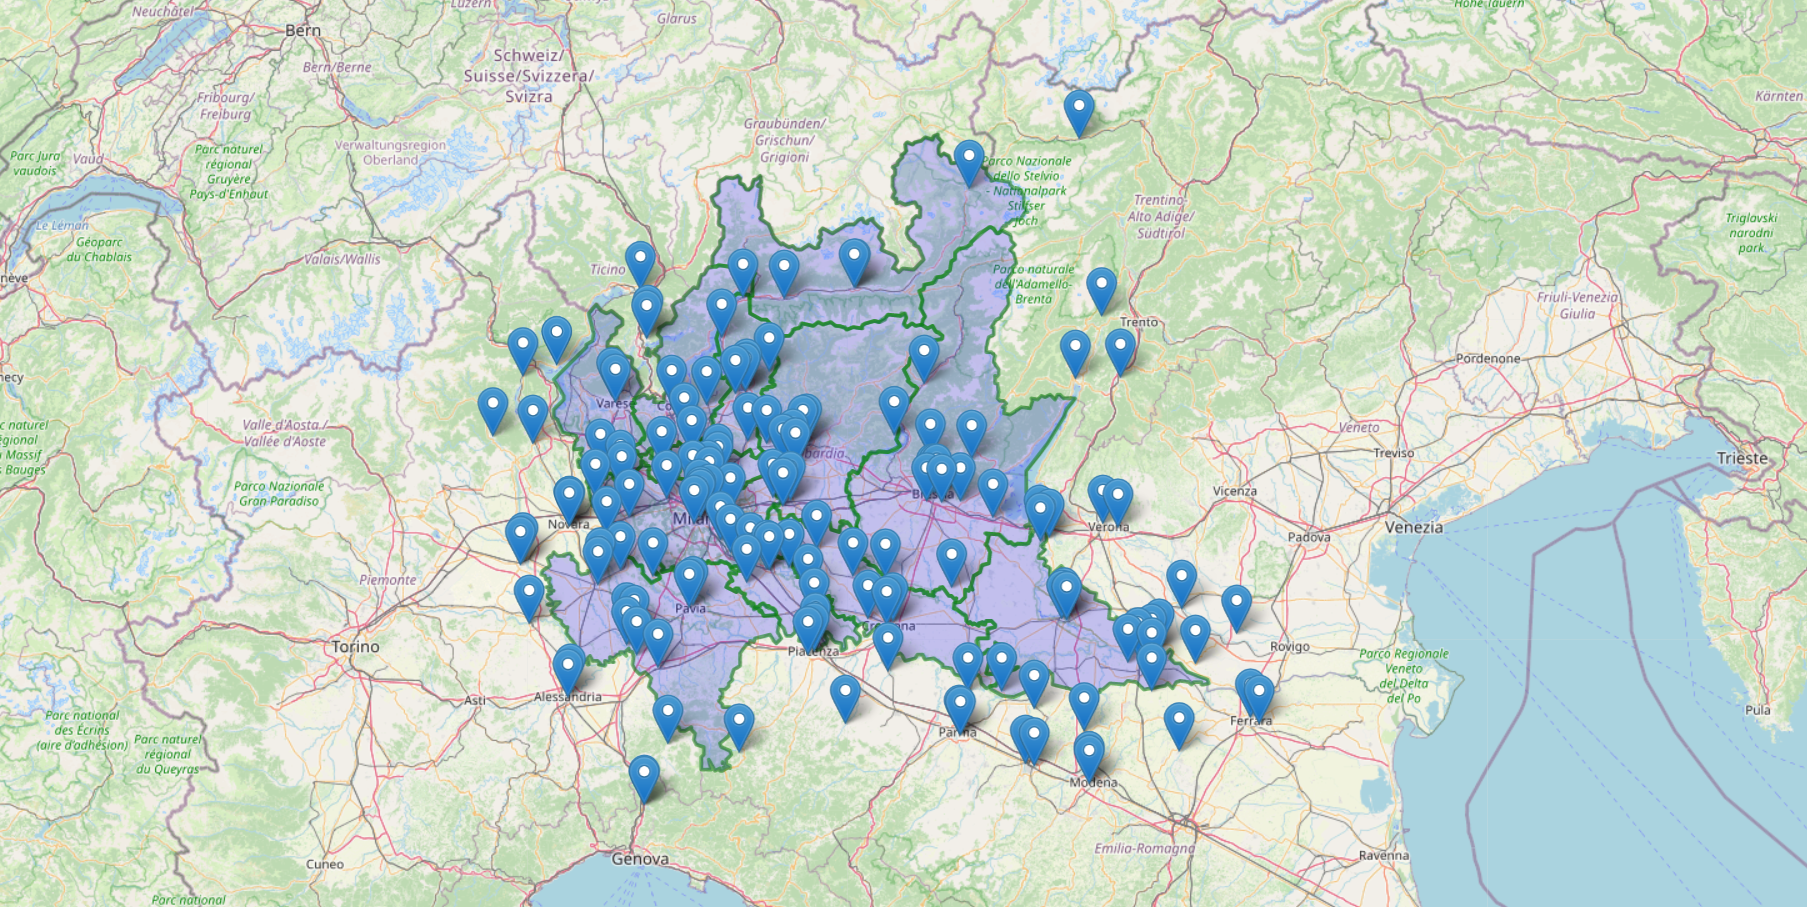
\includegraphics[width=0.8\textwidth]{./imgs/maps/mappa.png}
    \caption{Buffered Area around Lombardy Region}
    \label{fig:buffered_area}
\end{figure}
\textbf{Causes and sources related to the emissions:}
Particulate matter with a diameter of 2.5 micrometers or smaller originates from various anthropogenic and natural sources. Among the main causes related to the release of significant amounts of PM2.5 into the atmosphere, we can mention intensive livestock farming, as well as combustion processes, including those from vehicles and industrial activities.
Moreover, analyzing the provided dataset, it has emerged that one crucial variable influencing PM2.5 concentrations is the Boundary Layer Height (BLH) Max which represents the maximum depth of air next to the Earth's surface that is most affected by the resistance to the transfer of momentum, heat, or moisture across the surface. 

\begin{figure}[h]
    \centering
    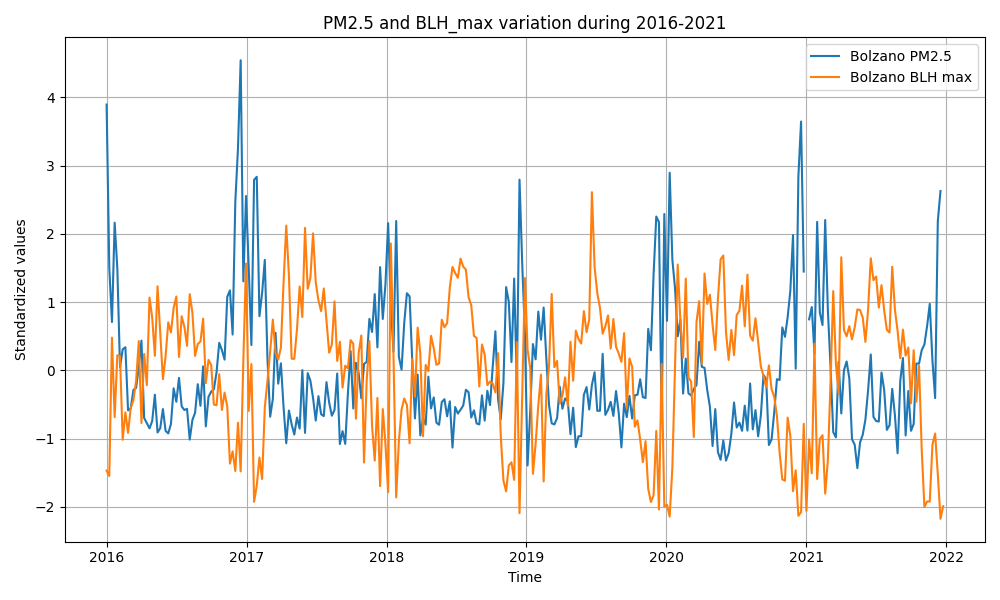
\includegraphics[width=0.8\textwidth]{./imgs/maps/plot_Bolzano_PM25_BLHmax_years.png}
    \caption{Correlation between PM2.5 Concentrations and Boundary Layer Height (BLH) max
     which represents the maximum depth of air next to the Earth’s surface that is most affected by the
    resistance to the transfer of momentum, heat, or moisture across the surface.}
    \label{fig:pm_blh_correlation}
\end{figure} 
\textbf{Main Problems Associated with PM2.5:}
In order to understand the relevance of the analysis developed in this project, it is important to focus on the problems and the risks associated with high concentrations of PM2.5
\begin{itemize}
    \item \textbf{Long Residence Time in the Atmosphere:} PM2.5 particles have an extended residence time in the atmosphere, leading to widespread dispersion and potential long-range transport. This characteristic contributes to the global distribution of PM2.5 and its diverse environmental impacts.

    \item \textbf{Health Impact:} Due to their small size, PM2.5 particles can penetrate deep into the human respiratory system, reaching the lungs and even entering the bloodstream. Prolonged exposure to elevated levels of PM2.5 is associated with various respiratory and cardiovascular diseases, posing a significant public health concern.

    \item \textbf{World Health Organization Recommendations:} The World Health Organization (WHO) recommends an \textbf{annual average} of $\leq 5\mu \frac{\mathrm{g}}{\mathrm{m}^3}$ for PM2.5 concentrations to safeguard public health. Exceeding these levels may lead to increased health risks, making it imperative to monitor and control PM2.5 pollution.
\end{itemize}

The outcomes of this analysis will not only enhance our understanding of PM2.5 variability but also assist policymakers and environmental scientists in formulating targeted interventions to mitigate the impact of air pollution on public health and the environment.


\section{Models}

Regarding the choice of models, we first focused on three basic modeling approaches: spatial-informed partitioning of the data, covariate-informed partitioning and modeling temporal dependence in partitions. Each of the modeling methods is a hierarchical model with Gaussian likelihood, a Gaussian prior for cluster-specific means and an uniform prior for cluster-specific variances. All of them allow for a number of specifications, e.g. different setting ups of priors. Later, several extensions and combinations were considered. \medskip

In the whole section we denote by $n$ the number of measurement units, by $\rho = \{ S_1, \dots, S_k \}$  a partition of the $n$ measurement units and by $c_i$ the cluster that measurement unit $i$ belongs to, i.e. $c_i = j$ if $i \in S_j$. Furthermore, cluster-specific values are marked with $*$. For example we consider cluster specific means $\pmb{\mu}^* = \{ \mu_1, \dots, \mu_k \}$ and standard deviations $\pmb{\sigma}^{*}$.

\subsection{sPPM Model: Spatial informed Clustering using location-dependent Similarity 
Functions} \label{subsec:sPPM-model}

The following model is taken from \cite{Page2016-Spatial}. It is implemented as part of the R-package \textit{ppmSuite} \cite{ppmSuite}.
The overall model structure is the following, where $m \in \RR, s^2 \in [0, \infty )$, the bounds $A, B \in [0, \infty)$ as well as the concentration parameter $M \in (0, \infty)$ and $\mathbf{\theta}$ that will be explained in more detail below are user-defined parameters.

\begin{align*}
    Y_i | \pmb{\mu}^*, \pmb{\sigma}^{2*}, c_i &\overset{\tiny{\mathrm{ind}}}{\sim} \Normal (\mu_{c_i}^*, \sigma_{c_i}^{2*}), i = 1, \dots, n \\
    (\mu_j^*, \sigma_j^*)  | \mu_0, \sigma_0^2 &\overset{\tiny{\mathrm{iid}}}{\sim} \Normal ( \mu_0, \sigma_0^2) \times \Uniform (0,A)\\
    (\mu_0, \sigma_0) &\sim \Normal (m, s^2) \times \Uniform (0,B)\\
    \rho &\sim \sPPM(M, \pmb{\theta})
\end{align*}

The $\sPPM$ is a prior of the following form, where $\mathbf{s}$ denotes the spatial coordinates of the measurement units:

\begin{align} \label{sPPM-prior}
    \PP(\rho | \pmb{s} ) \propto \prod_{j=1}^{k_{\rho}} \left( \underbrace{M \cdot \Gamma(\vert S_j \vert) }_{=:c(S_j)}g(S_j, \pmb{s}^*_j \vert \pmb{\theta}) \right) .
\end{align}

The so-called similarity function $g$ is a non-negative function that measures the togetherness of the stations in the set $S_j$.
Note that $\prod_{j=1}^{k_{\rho}} c(S_j) $ is proportional to the distribution of $\rho$ in a random partition model induced by a sample from a Dirichlet process (Section 8.1.3 in \cite{lecturenotes}). Therefore $M$ takes the role of the concentration parameter in the Dirichlet process and influences the number of clusters.\medskip

For the similarity function $g$ that incorporates the spatial information there are four options available. \medskip

\begin{enumerate}
    \item $\theta = \alpha \in (0,\infty)$ with the distance measure
    \begin{align*}
        g_1(S_j, \pmb{s}_j^* \vert \theta) := \begin{cases}
            \frac{1}{\Gamma(\alpha \DD_h) \indicator[\DD_h \geq 1] + \DD_h \indicator[\DD_h < 1]}, &\quad \text{ if } \vert S_h \vert > 1\\
            M, &\quad \text{ if } \vert S_h \vert = 1
        \end{cases}
    \end{align*}
    with a distance function $\DD_h := \sum_{i \in S_h} d(\pmb{s}_i, \bar{\pmb{s}}_h)$ and the cluster centroid
    $\bar{s}_{hk} = \frac{1}{n_h} \sum_{i\in S_h} s_{ik}$ for coordinates $k=1,2$ and $n_h := \vert S_h \vert$. Larger $\alpha$ favors denser clusters.  \medskip
    
    \item $\theta = a \in (0, \infty)$ with distance measure
    \begin{align*}
        g_2(S_h, \pmb{s}_h^* \vert \theta) := \prod_{i, j \in S_h} \indicator\left[\lVert s_i - s_j\rVert \leq a \right].
    \end{align*}
    Larger $a$ allows for larger neighborhoods. \medskip
    
    \item  \textit{(Auxiliary Cohesion)} With dimension $d=2$ and
    $\pmb{\xi} = (\pmb{m}, \pmb{V}) \in \RR^d \times \PosSemDef_+^d = \RR^d \times \{X \in \RR^{d\times d} \vert X \succeq 0\} =: \Xi$, we have (prior predictive conjugate model)
    \begin{align*}
        g_3(S_h, \pmb{s}_h^* \vert \pmb{\theta}) := \int_{\Xi} \prod_{i \in S_h} q(\pmb{s}_i \vert \xi_h) q(\xi_h) \dd \xi_h
    \end{align*}
    with $q(\pmb{s}\vert \pmb{\xi}) = \Normal(\pmb{s}\vert \pmb{\xi})$ and $q(\pmb{\xi}) = \NormInvWish(\pmb{m}, \pmb{V} \vert \pmb{\mu_0}, \kappa_0, \nu_0, \Delta_0 \cdot \Identity_d)$
    for user-defined parameters 
    $\pmb{\theta} = \left(\pmb{\mu_0}, \kappa_0, \Delta_0, \nu_0\right) \in \RR^d \times (0, \infty)^2 \times (1, 
    \infty)$ (last part since $\nu_0 > d -1$ has to be fulfilled) \medskip
    
    \item \textit{(Double Dipper)} With same structure as $g_3$, but with a posterior predictive conjugate model
    \begin{align*}
        g_4(S_h, \pmb{s}_h^* \vert \pmb{\theta}) := \int_{\Xi} \prod_{i \in S_h} q(\pmb{s}_i \vert 
        \xi_h) q(\xi_h\vert \pmb{s}_h^*) \dd \xi_h
    \end{align*}
    and conjugate model $q(\pmb{s}_i \vert 
        \xi_h) = \Normal(\pmb{s}_i \vert \pmb{m}_h, \pmb{V}_h)$ and $q(\xi_h\vert \pmb{s}_h^*) = 
        \NormInvWish(\pmb{m}_h, \pmb{V}_h \vert \pmb{s}_h^*)$
    Compared to $g_3$ this option is more peaked and puts more weights on local partitions.
\end{enumerate}


\subsection{PPMx: Clustering using Covariate-dependent Similarity functions and Prior on Cluster Size}

The covariate-informed partition model is taken from \cite{Page2017-Covariate} and all the introduced variants are implemented in the $R$-package \ppmSuite{} \cite{ppmSuite}. The overall structure is the same as for the spatial-informed clustering with the difference that the similarity function now measures the homogeineity of the covariate values in a given partition set. Again, the values $m \in \mathbb{R}, s^2 \in [0, \infty)$ and bounds $A, B \in [0, \infty )$ as well as concentration parameter $M \in (0, \infty)$ and parameter(s) $\theta$ for the chosen similarity function are user-defined.
\begin{align*}
    Y_i \vert \pmb{\mu}^*, \pmb{\sigma}^{2*}, c_i \overset{\tiny{\mathrm{ind}}}&{\sim} \Normal (\mu_{c_i}^*, \sigma_{c_i}^{2*}), i = 1, \dots, n \\
    % (\mu_j^*, \sigma_j^*)  | \mu_0, \sigma_0^2 \overset{\tiny{\mathrm{iid}}}&{\sim} \Normal ( \mu_0, \sigma_0^2) \times \Uniform (0,A)\\
    % (\mu_0, \sigma_0) &\sim \Normal (m, s^2)\times \Uniform (0,B)\\
    % \rho &\sim \PPMx(M, \pmb{\theta})
\end{align*}
The prior for the clusters is
\begin{align*}
    \PP(\rho | \pmb{x} ) \propto \prod_{j=1}^{k_{\rho}} c(\vert S_j \vert)g(\pmb{x}^*_j \vert \pmb{\theta}).
\end{align*}
For the so-called cohesion function $c$ either the same function as in \Cref{sPPM-model} (that is proportional to the partition probabilities in a random partition model derived from a Dirichlet process), or a uniform cohesion $c \equiv 1$ can be chosen. \medskip

In the following discussion $p=1$ is assumed if not stated otherwise. If $p$ covariates are available, in general
\begin{align*}
    \Tilde{g}(\pmb{x}_j^* \vert \pmb{\theta} ) = \prod_{l=1}^p g(\pmb{x}_{jl}^* \vert \pmb{\theta})
\end{align*}
is adopted.\medskip

As a large number of covariates can lead to either a large number of singleton clusters or one single cluster, there are two optional methods to cap the influence of the covariates on the partitioning.

\begin{align*}
    (1) \ \Tilde{g} (\pmb{x}_j^*) = \frac{g (\pmb{x}_j^*)}{\sum_{i=1}^{k_j} g(\pmb{x}_i^*)} \ \text{\ \ or \ \ } \ (2) \ \Tilde{g} (\pmb{x}_j^*) = g (\pmb{x}_j^*)^{\frac{1}{p}}
\end{align*}

For similarity functions $g$ there are four options available.\medskip

\begin{enumerate}
 \item With $\theta = \alpha \in (0, \infty)$
    \begin{align*}
        g_1( \pmb{x}_j^* \vert \theta ) := \exp{- \alpha H (\pmb{x}_j^*) }.
    \end{align*}
    For continuous covariates $
    H(\pmb{x}_j^*)= \frac{1}{n} \sum_{l \in S_j} (x_l - \overline{x}_j)^2$ and for categorical covariates $H(\pmb{x}_j^*)= \sum_{c=1}^C \hat{p}_{cj} \log{\hat{p}_{cj}}$, where $C$ is the number of categories and $\hat{p}_{cj}$ the proportion of observations in category $c$ in cluster $j$.
    Higher values of $\alpha$ lead to an increased penalty for dissimilar covariate values. Extensions to the multivariate case are possible (determinant of cluster-specific covariate matrices or multivariate entropy respectively). \medskip

    \item For any number of covariates $p$ and penalty $\theta = \alpha \in (0, \infty)$

    \begin{align*}
        g_2( \pmb{x}_j^* \vert \theta) &:= \exp{- \alpha \sum_{i,k \in S_j, i \neq k} d(\pmb{x}_i, \pmb{x}_k ) }
    \end{align*}
    and
    \begin{align*}
        g_3( \pmb{x}_j^* \vert \theta) &:= \exp{- \frac{2 \alpha}{n_j (n_j - 1)} \sum_{i,k \in S_j, i \neq k} d(\pmb{x}_i, \pmb{x}_k ) }
    \end{align*}
    are based on the Gower Dissimilarity:
    \begin{align*}
        d(x_{il}, x_{jl}) := \begin{cases}
            \frac{\vert x_{il} - x_{jl} \vert}{\max_h x_{hl} - \min_h x_{hl}}, &\quad \text{ if } l \text{-th cov. continuous}\\
            \delta_{x_{il} x_{jl}}, &\quad \text{ if } l \text{-th cov. categorical}
        \end{cases}
    \end{align*}
    and $d(\pmb{x}_i, \pmb{x}_k )$ is the average of the Gower Dissimilarities in the $p$ components. \medskip

    \item  \textit{(Auxiliary Similarity Function)} With an auxiliary parameter
    $\pmb{\xi}_j^*$, we have (prior predictive conjugate model)
    \begin{align*}
        g_4(\pmb{x}_j^* \vert \pmb{\theta}) := \int \prod_{i \in S_j} q(x_i \vert \pmb{\xi}^*_j) q(\pmb{\xi}^*_j) \dd \pmb{\xi}^*_j
    \end{align*}
    
    For continuous covariates there are two options as a conjugate model. First, the \textit{Auxiliary N-N Model} with $q(. \vert \xi_j^*) = \Normal (. \vert \xi_j^*, \kappa_1 \hat{S})$  and $q(\xi_j^*) = \Normal (\xi_j^* \vert m_0, s_0^2)$ where $\hat{S}$ denotes the empirical variance of the covariate. The user-supplied parameters are $\pmb{\theta} = ( \kappa_1, m_0, s_0).$ Second, the \textit{Auxiliary N-NIG Model} with $q (. \vert \pmb{\xi_j^*}) = \Normal(. \vert m_j^*, v_j^*)$ and $q(\pmb{\xi}_j^*) = \text{N-IG} (m_j^*, v_j^* \vert m_0, k_0, v_0, n_0)$. The user-supplied parameters are $\pmb{\theta} = (m_0, k_0,v_0, n_0)$. \medskip
    
    For categorical covariates a Multinomial-Dirichlet Model is applied, that is \newline $q(. \vert \pmb{\xi}_j^*) = \Multinomial ( . \vert \pmb{\xi}_j^* )$ and $q( \pmb{\xi}_j^*) = \Dir ( \pmb{\xi}_j^* \vert \pmb{\alpha}_j \equiv a )$ where $C$ is the number of cateogories. The user-supplied parameter is $\theta = a$. \medskip

    \item \textit{(Double Dipper)} With an auxiliary parameter
    $\pmb{\xi}_j^*$, we have
    \begin{align*}
        g_5(\pmb{x}_j^* \vert \pmb{\theta}) := \int \prod_{i \in S_j} q(x_i \vert \pmb{\xi}^*_j) q(\pmb{\xi}^*_j \vert \pmb{x}_j^*) \dd \pmb{\xi}^*_j
    \end{align*}

    with the same options for the underlying models as for $g_4$. This option gives more weight on the local covariate structure compared to $g_4$. 
\end{enumerate}

\subsection{DRPM Model: Dependent Modeling of Temporal Sequences of Random Partitions}

In this model that is taken from \cite{Page2021-Temporal} and is implemented in the $R$-package \drpm{} \cite{drpm} finally a temporal evolvement of the partitions is considered. The overall model structure is the following:

\begin{align*}
    Y_{it} \vert \pmb{\mu}^*_t, \pmb{\sigma}^{2*}_t, \mathbf{c}_t
    \overset{\tiny{\textrm{ind}}} &{\sim} \Normal({\mu}^*_{c_{it}t}, 
    {\sigma}^{2*}_{c_{it}t}) \quad \forall i=1,\ldots,n; \, t=1,\ldots, T\\
    (\mu_{j t}^*, \sigma_{jt}^*) \vert \theta_t, \tau_t^2 
    \overset{\tiny{\textrm{ind}}} &{\sim} \Normal(\theta_t, \tau_t^2) \times \Uniform(0, A_\sigma) \quad \forall j=1,\ldots, k_t\\
    (\theta_t, \tau_t) \overset{\tiny{\textrm{iid}}} &{\sim}\Normal(
    \phi_0, \lambda^2) \times \Uniform\left(0, A_\tau\right) \quad \forall t=1, \ldots, T\\
    (\phi_0, \lambda) &\sim \Normal(m_0, s_0^2) \times \Uniform(0, A_\lambda) \\
    \{ \pmb{c}_1, \ldots, \pmb{c}_T\} &\sim \tRPM(\pmb{\alpha}, M) \; \textrm{with} \; \alpha_t \iid{} \BetaDist(a_\alpha, b_\alpha).
\end{align*}

The temporal random partition model models the temporal sequence of clusters as a first-order Markovian structure. We denote the clusters as $\rho_t = \{S_{1t}, \ldots, S_{k_t, t}\}$, $t=1, \ldots, T$ or use the cluster-labeling notation. 

The first ingredient for the model is an exchangeable probability function (EPPF) on the set of partitions of the measurement units. In our case
\begin{align*}
    \text{P} (\rho\vert M) = \frac{M^{k_\rho}}{\prod_{i=1}^n (M+i-1)} \prod_{i=1}^{k_\rho} \left( \vert S_i\vert -1\right)!
\end{align*}
is applied. This is the marginal probability function for $\rho$ derived from a Chinese Restaurant process with concentration parameter $M$. Smaller $M$ favors less but larger clusters. This function is the prior for $\rho_1$.
 
Secondly, in order to define transition probabilities an auxiliary parameter $\mathbf{\gamma}_t$ is introduced. We define $\gamma_{it} \sim \Bernoulli(\alpha_t)$, i.e. 
$\gamma_t \in \{0,1\}^{\#\text{stations}}$ and give the following interpretation:

\begin{align*}
    \gamma_{it} = \begin{cases}
        1, \; \text{station } i \text{ is \textbf{not} relocated when moving from time } t-1 \text{ to } t\\
        0, \; \text{else}
    \end{cases}.
\end{align*}
The values of $\alpha_t \in [0,1]$ regulate the time-dependency, e.g. $\alpha_t = 1$ means $\rho_t = \rho_{t-1}$ with probability 1 and $\alpha_t = 0$ implies $\rho_t$ is independent of $\rho_{t-1}$. \medskip

Given $\gamma_t$ and $\rho_{t-1}$ there is restriction to what partitions are compatible and can be considered for $\rho_{t}$. The transition probabilities are then
\begin{align*}
    \PP(\gamma_1, \rho_1, \ldots, \gamma_T, \rho_T) = \PP(\rho_T\vert \gamma_T, \rho_{T-1})  \cdots  \PP(\rho_2\vert \gamma_2, \rho_{1}) \PP(\rho_1)
\end{align*}
and for $t \in \{1, \dots, T \}$ the $\PP(\rho_t\vert \gamma_t, \rho_{t-1})$ is given by the chosen EPPF from before truncated to the set of compatible partitions.

% IMPORTANT: do not remove this chapter, as references depend on it
\subsection{Extensions}
\label{subsec:DRPMExtensions}

For the DPRM Model we considered the extensions listed below. All of them were available in the \textit{drpm} package \cite{drpm}. The full extended model is taken from section 4 in \cite{Page2021-Temporal}. \medskip

?? Does not really match with drpm package: in the package $\eta_1, \phi_1$ are updated??; we can provide a scale prior for xi?; we cannot set $\phi_1$? :(

\textbf{Fixed $\alpha$ for each time step}\\
Instead of drawing an $\alpha_t$ in each time step, we considered using a constant, user-supplied $\alpha_0$ (?) for the probability of non-relocation for each measurement unit. To be precise this is not an extension, but was considered as we wanted to see if the resulting models are worse and if they run significantly faster. \medskip

\textbf{Unit, i.e. station, specific $\alpha$ values}\\ -- adjust the prior size accordingly \medskip


\textbf{Spatially informed DRPM}\\
This extension combines the DRPM and the sPPM model. The EPPF in the temporal random partition model is changed to the function that was used as a prior in the sPPM-model, i.e. \ref{sPPM-prior}. For similarity functions \textit{Auxiliary Cohesion} and \textit{Double Dipper} ($g_3$ and $g_4$ in section \ref{subsec:sPPM-model}) were considered. (In section 4.1 of \cite{Page2021-Temporal} it is stated [...] that when standardizing the spatial coordinates and setting $\mathbf{\mu_0} = \mathbf{0}, \kappa_0 = 1$ and $\Delta_0 = 1$ for the NIW-parameters in $g_3$, we get a EPPF that preserves sample size consistency. In this case larger $\nu_0$ implies larger influence of spatial data on the clustering) \medskip

\textbf{AR(1) structure in the Likelihood}\\
As it is reasonable to assume that there is a temporal dependence for the time series at each measurement unit, a temporal structure in the likelihood is considered. For that purpose a measurement-unit specific time dependence parameter $\eta_i$ with $|\eta_i| \leq 1$ is introduced. The resulting model is obtained when setting $\phi_1 = 0$ in the model presented below.
%AR(1)-method using eta not equal to zero (otherwise iid)
\medskip

\textbf{AR(1) structure for $\theta_t$}\\
In addition a time-dependency in the time specific means $\theta_t$ can be added by bringing in another parameter $\phi_1$. Together with the AR(1) structure in the likelihood the extended model the following.
\begin{align*}
    Y_{it} \vert \pmb{\mu}^*_t, \pmb{\sigma}^{2*}_t, \mathbf{c}_t
    \overset{\tiny{\textrm{ind}}} &{\sim} \Normal({\mu}^*_{c_{it}t} + \eta_i Y_{i t-1}, 
    {\sigma}^{2*}_{c_{it}t}(q-\eta_i^2)) \quad \forall i=1,\ldots,n; \, t=1,\ldots, T\\
    Y_{i1} \overset{\tiny{\textrm{ind}}} &{\sim} \Normal ({\mu}^*_{c_{i1}1}, {\sigma}^{2*}_{c_{i1}1}) \quad \forall i=1,\ldots,n\\
    \xi_i = \text{Logit}(0.5(\eta_i + 1)) \overset{\tiny{\textrm{iid}}} &{\sim} \Laplace (a,b) \quad \forall i=1,\ldots,n\\
    (\mu_{j t}^*, \sigma_{jt}^*) \vert \theta_t, \tau_t^2 
    \overset{\tiny{\textrm{ind}}} &{\sim} \Normal(\theta_t, \tau_t^2) \times \Uniform(0, A_\sigma) \quad \forall j=1,\ldots, k_t;  t=1,\ldots, T\\
    \theta_t | \theta_{t-1} \overset{\tiny{\textrm{ind}}} &{\sim} \Normal ((1- \phi_1) \phi_0 + \phi_1 \theta_{t-1}, \lambda^2 (1- \phi_1^2))\\
    (\theta_1, \tau_t) &\sim  \Normal(
    \phi_0, \lambda^2) \times \Uniform\left(0, A_\tau\right) \quad \forall t=1, \ldots, T\\
    (\phi_0, \phi_1, \lambda) &\sim \Normal(m_0, s_0^2) \times \Uniform (-1,1) \times \Uniform(0, A_\lambda)\\
    \{ \pmb{c}_1, \ldots, \pmb{c}_T\} &\sim \tRPM(\pmb{\alpha}, M) \; \textrm{with} \; \alpha_t \iid{} \BetaDist(a_\alpha, b_\alpha).
\end{align*}



Note that setting $\eta_i = 0$ and $\phi_1 = 0$ this model is exactly the DRPM model from before.
%phi value 0 value corresponds to independent atom


\section{Data Preparation and Evaluation}


\subsection{The Agrimonia Database}

\subsection{Data Exploration}
TODO: show the correlation plot, show time series over different years
list data loss, number of stations

\subsection{Imputation of Missing Data}

\subsection{Data Aggregation}

\subsection{Evaluation}

\subsubsection{Goodness-of-fit}
To indicate goodness-of-fit of the used models the following criteria are considered.

\textbf{LPML = log pseudo marginal likelihood} (higher is better)
The LPML is a predictive information criterion based on the idea of leave-on-out cross validation \cite{lecturenotes}. Let $\mathbf{y} = (y_1, \dots , y_n )$ denote our data, $\mathbf{y}_{(-i)} = (y_1, \dots , y_{i-1}, y_{i+1}, \dots, y_n )$ and $m(y_i | \mathbf{y}_{(-i)}) $ the marginal likelihood of $y_i$ given $\mathbf{y}_{(-i)}$ in the considered model. Then the LPML is defined as
\begin{align*}
    \text{LPML} = \sum_{i=1}^n \log m(y_i | \mathbf{y}_{(-i)}).
\end{align*}
    
\textbf{WAIC = widely applicable information criterion} (lower is better)
The WAIC is another predictive information criteria that accounts for the over-estimation of log pointwise predictive density $\sum_{i=1}^n \log m(y_i | \mathbf{y})$ by subtracting a penalization term $p_{WAIC}$ \cite{lecturenotes}. In our definition the WAIC is obtained by multiplying this difference with $-2$. In the following $\mathbf{\theta}$ denotes the parameters and $f$ the likelihood of the given model. The WAIC is defined as
\begin{align*}
    \text{WAIC} &= -2 \left( \sum_{i=1}^n \log m(y_i | \mathbf{y} ) - 
    p_{\text{WAIC}} \right), \\
    p_{\text{WAIC}} &= \sum_{i=1}^n \text{Var}_{\theta | \mathbf{y}} \log 
    f(y_i | \mathbf{\theta} ).
\end{align*}

\textbf{MSE = mean squared error} (lower is better)
Denote by $\hat{y}_i = \mathbb{E}(Y_i | \mathbf{y})$ the posterior mean of the $i$-th observation, then
\begin{align*}
    \text{MSE} = \frac{1}{n} \sum_{i=1}^n (y_i - \hat{y}_i)^2.
\end{align*}

\textbf{MaxDev = Maximal Deviation} (lower is better)
Given a partition $\rho
= \{S_1, \ldots, S_k\}$ we compute the maximum of the cluster-internal 
deviation of PM2.5 values over all cluster, namely
\begin{align*}
    \text{MaxDev} = \max_{i=1, \ldots, k} \left(\max_{i\in S_k} y_i - 
    \min_{i\in S_k} y_i
     \right)
\end{align*}
as an indication on how closely related the target variable's
values are given the partition $\rho$.


\subsubsection{Predictive Performance}
The predictive performance of the models is measured by the mean squared prediction error.

\textbf{MSPE = mean squared prediction error} (lower is better)\\
Denote by $\Tilde{y}_i$ the testing observation for the $i$-th measurement unit, then
\begin{align*}
    \text{MSPE} = \frac{1}{n} \sum_{i=1}^n (\Tilde{y}_i - \hat{y}_i)^2.
\end{align*}

\subsubsection{Cluster estimation}
Once a model is fit to the data the question remains how to summarize the obtained posterior for the clusters in a meaningful way. One number that we report is the posterior mean of the number of clusters. Furthermore, a general idea is to find an estimate $\hat{\rho}^*$ that minimizes a certain partition loss function $L$. Assuming that there is a ``true'' $\rho$ (we take the posterior distribution), this becomes
\begin{align*}
    \hat{\rho}^* = \text{argmin}_{\hat{\rho}} \ \mathbb{E} ( L(\rho, \hat{\rho}) | \mathbf{y} ) \approx \frac{1}{M} \sum_{m=1}^M L (\rho^{(m)} , \hat{\rho} ),
\end{align*}
where $\left( \rho^{(1)}, \dots , \rho^{(M)} \right)$ are MCMC samples from the posterior. For that approach the $R$-package \texttt{salso} \cite{salso} provides a number of possibilities. In \cite{Dahl2022-salso} different loss functions are explained as well as the \texttt{SALSO} algorithm that is implemented in the package.

\textbf{Binder Loss} One of the most widely used loss functions is the Binder loss function that considers pairwise misclassifications. Switching to the equivalent cluster notation for partitions the definition is
\begin{align*}
    \text{L}_{\text{Binder}} (\mathbf{c}, \mathbf{\hat{c}} ) = \sum_{i<j} a \cdot  I (\{ c_i = c_j \}) I (\{ \hat{c_i} \neq \hat{c_j} \} ) +  b \cdot I (\{c_i \neq c_j \}) I (\{ \hat{c_i} = \hat{c_j} \}).
\end{align*}
For $a=b=1$ a measure of similarity between partitions, the Rand Index, is obtained by $\text{RI}(\rho, \hat{\rho}) = 1 -  \text{L}_{\text{Binder}}(\rho, \hat{\rho}) / \binom{n}{2}$. Maximizing the the posterior expectation of the Rand Index is equivalent to minimizing the expected loss for a Binder loss function with $a=b=1$. As this index fails to account for chance agreements, there exists a generalization that we will consider.

\textbf{Adjusted Rand Index} The Adjusted Rand Index (ARI) is defined as
\begin{align*}
    \text{ARI} (\rho, \hat{\rho}) = \frac{ \sum_{s \in \rho} \sum_{E \in \hat{\rho}} \binom{| S \cap E |}{2} - \left( \sum_{S \in \rho} \binom{|S|}{2} \sum_{E \in \hat{\rho}} \binom{|E|}{2} \right) \frac{1}{\binom{n}{2}}} {\frac{1}{2} \left( \sum_{S \in \rho} \binom{|S|}{2} + \sum_{E \in \hat{\rho}} \binom{|E|}{2} \right) - \left(\sum_{S \in \rho} \binom{|S|}{2} \sum_{E \in \hat{\rho}} \binom{|E|}{2} \right) \frac{1}{\binom{n}{2}}}.
\end{align*}
Large values mean a larger similarity between the partitions. We obtain another point estimate of the posterior expectation of the partition by maximizing the posterior expectation of the ARI.

\newpage

\section{Results}
We used the same seed for every experiments to make the results
reproducible and comparable
\subsection{sPPM}
\subsection{PPMx}
\subsection{DRPM}
\subsubsection{Non-spatially informed: Hyperparameter Gridsearch}
In order to test the model's sensitivity and response with respect to different values of the hyperparameters $M$ and the starting value
$\alpha_0$ we provide a large grid-search-like experiment. To investigate the model's dependency on different values of the prior parameters,
we conduct each of the grid-search-like experiment for three different prior believes presented in \cref{tab:DRPMPriorParam}. The first
prior values, namely DRPM-Paper, are directly taken from \cite[Section 4.1]{Page2021-Temporal} in the context of monthly PM10 data
and we consider this model as a baseline. Since our early explorations showed that these prior parameters lead to quite large clusters
(most of the times the model only returned one or two clusters), we modified the prior values to incorporate a lower standard deviation
for the likelihood, nameley Lower Std, and we provide a third set of prior values which additionally integrate the mean PM2.5 value
of the year 2018 as a prior value for the predictive mean. To make the experiments comparable and reproducable, we use the same
random see for each of the experiments.

The results are comprehensively available in the folder \texttt{/report/tables/results} of the Github
repository.\footnote{See \url{https://github.com/Flo-Wo/PM25-Clustering/tree/main/report/tables/results}}
For the sake of simplicity and limited space available, we only present the best hyperparameters for each of the model
in the summary \cref{tab:DRPMNoSpatialSummary}. Interestingly, as already mentioned, the baseline model using the 
DRPM-Paper prior values performs poorly and, as shown in \cref{fig:drpm_base_models_comparison}, all stations are in
the same cluster for each time step. In contrast, the models using our two tuned prior values perform reasonably well,
despite requiring longer computational times of factor 5 and 7 respectively, most probably due to a less informative
prior on the $\alpha_t$ values. Additionally, we were surprised that the WAIC and MSE performance metrics do not correlate.
Notwithstanding looking promising on paper with the lowest MSE of $1.271$, the DRPM-Paper informed model performs poorly in practice,
as it is obvious that a clustering of all stations in one cluster is absolutely not desirable. Consequently, despite having
an higher MSE, our prior values are favorable. An exemplary clustering of the three models is visualized in 
\cref{fig:DRPMClusteringBaseModels}. In \cref{fig:drpm_base_models_comparison} we analyzed the three different models
with respect to their number and sizes of clusters. Although the time-evolvement of $\alpha_t$ is somehow similar for all
three models, the number of clusters significantly differ and the mean-informed Mean 2018 version favors slighly more
clusters than the zero-centered mean version Lower Std. The MSE of the model using our two priors is nearly equal.

In order to analyze the convergence behaviour of the MCMC, we exemplarily visualize trace plots for the parameters of
our Lower Std prior model, as it was the best performing one in our initial test. The plots in
\cref{fig:drpm_lower_std_trace_plots} clearly exhibit the desirable \enquote{fat caterpillar} structure for the
parameters $\mu^*_{c_1t}$, $\tau_t^2$ and $\phi_0$, nonetheless for the rest of the shown parameters the convergence
behaviour could be improved. Given the results presented in \cite[Section 4.1]{Page2021-Temporal} with 50.000 MCMC samples,
we expect this behaviour to vanish when increasing the number of samples as well as the burn-in and the thinning.

\begin{table}[h]
\centering
\begin{tabular}{lcccccccc}
\toprule
Name $\setminus$ Prior Parameters & $m_0$ & $s_0^2$ & $A_\sigma$ & $A_r$ & $A_\lambda$ & $b$ & $a_\alpha$ & $b_\alpha$ \\
\midrule
DRPM-Paper \cite{Page2021-Temporal} & 0.0   & $100^2$ & 10.0         & 5.0     & 5.0           & 1.0   & 2.0        & 2.0        \\
Lower Std (ours)                                & 0.0   & $200$   & 0.1        & 1.0     & 1.0           & 1.0   & 1.0          & 1.0          \\
Mean 2018 (ours)                                & 2.91  & $200$  & 0.1        & 1.0     & 1.0           & 1.0   & 1.0          & 1.0         \\
\bottomrule
\end{tabular}
\caption{Different Prior Parameters for the three models we used for our initial large test.}
\label{tab:DRPMPriorParam}
\end{table}

\begin{table}
\caption{Non-spatially informed DRPM model performances for different prior values. A dash value indicates that the \texttt{drpm$\_$fit} function
was not able to compute the corresponding values due to unknown reasons. Bold values indicate the column-wise best result.}
\centering\begin{tabular}{cccccccccccc}
\toprule
Prior & M & $\alpha_0$ & LPML & WAIC & Time [s] & MSE & MaxDev \\
\midrule
DRPM-Paper & 100.0& 0.25& $-1.234 \cdot 10^{+03}$ & $2.445 \cdot 10^{+03}$ & $\mathbf{12.70} $ & $\textbf{1.271}$ & $1.753$ \\
Lower Std & 0.1& 0.25& $-$ & $\mathbf{-1.285 \cdot 10^{+03}}$ & $68.71 $ & $1.696 $ & $\textbf{1.495}$ \\
Mean 2018 & 0.1& 0.25& $-$ & $-9.548 \cdot 10^{+02}$ & $90.26 $ & $1.699 $ & $1.679$ \\
\bottomrule
\end{tabular}
\label{tab:DRPMNoSpatialSummary}
\end{table}


\begin{figure}
    \centering
    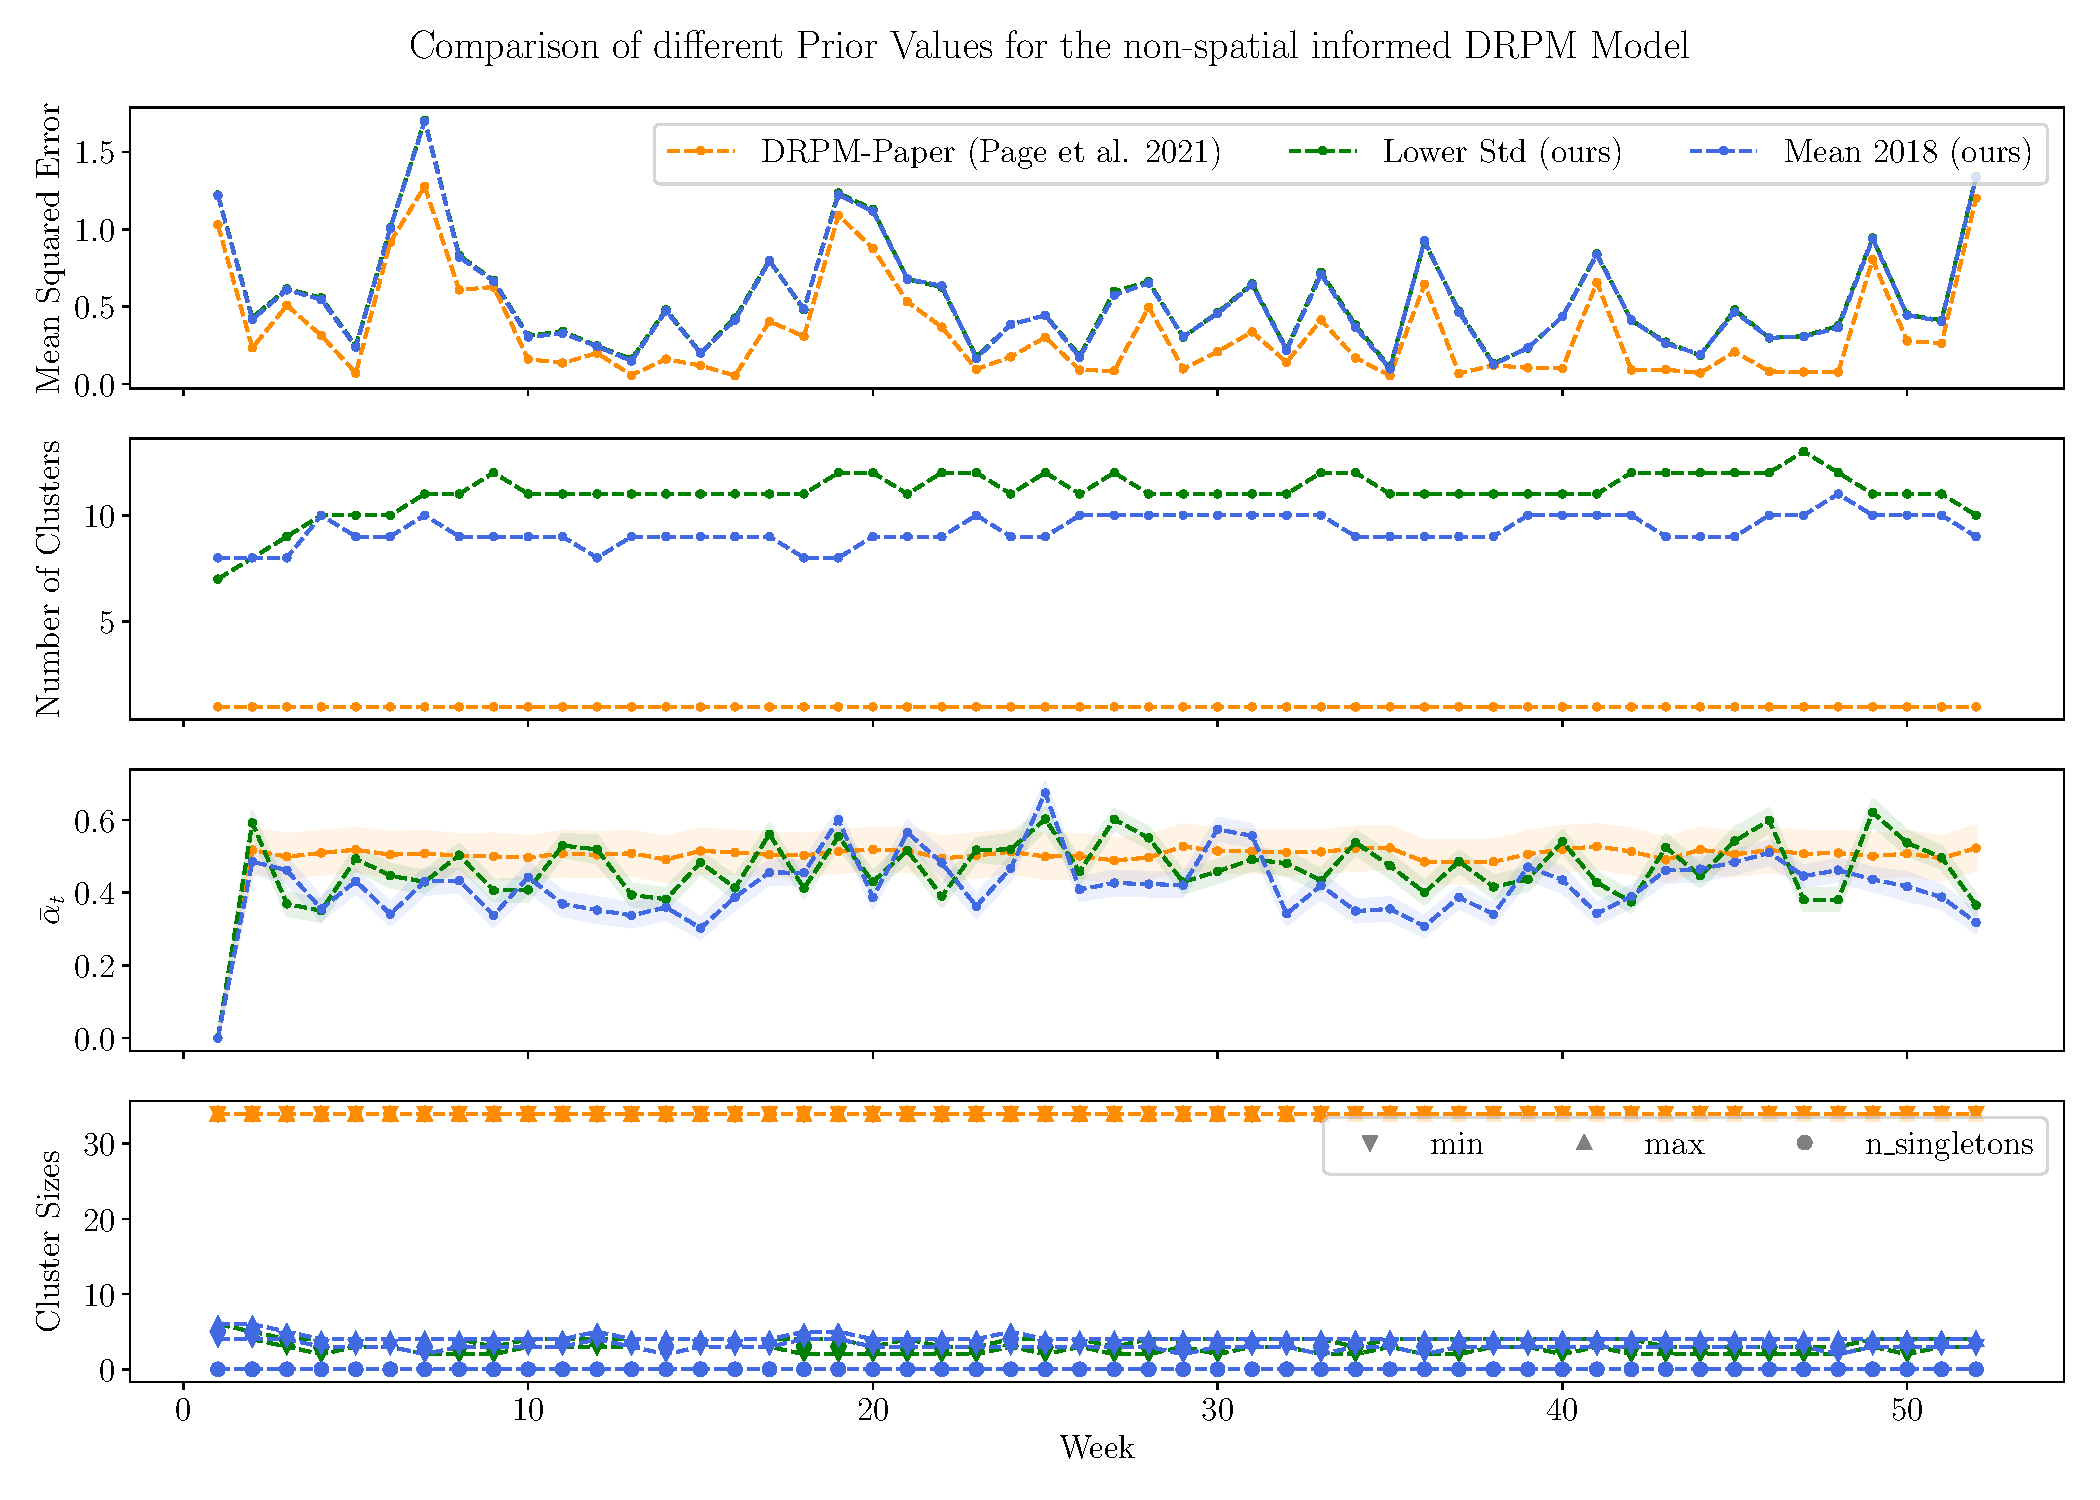
\includegraphics[width=.95\linewidth]{./imgs/drpm/drpm_base_models_comparison.pdf}
    \caption{Comparison of the best model for each prior for DRPM without spatial cohesion.
    The used prior values are listed in \cref{tab:DRPMPriorParam}. For the DRPM model itself we use
    $M=0.1$ as the concentration parameter. The MCMC uses 10000 draws with a burn-in of 1000 and a
    thinning of 10, resulting in 900 total MCMC samples. The DRPM-Paper model reached a WAIC (lower is better) of
    $3.103 \cdot 10^{+03}$ while our models achieved a WAIC score of $-1.285 \cdot 10^{+03}$ and
    $-9.548 \cdot 10^{+02}$ for the Lower Std and Mean 2018 models respectively. For the cluster sizes,
    the minimum (min) and maximum (max) number of stations for each timestep is shown, as well as the number of
    singletons, i.e. clusters consisting of only one station.}
    \label{fig:drpm_base_models_comparison}
\end{figure}

\begin{figure}
    \centering
    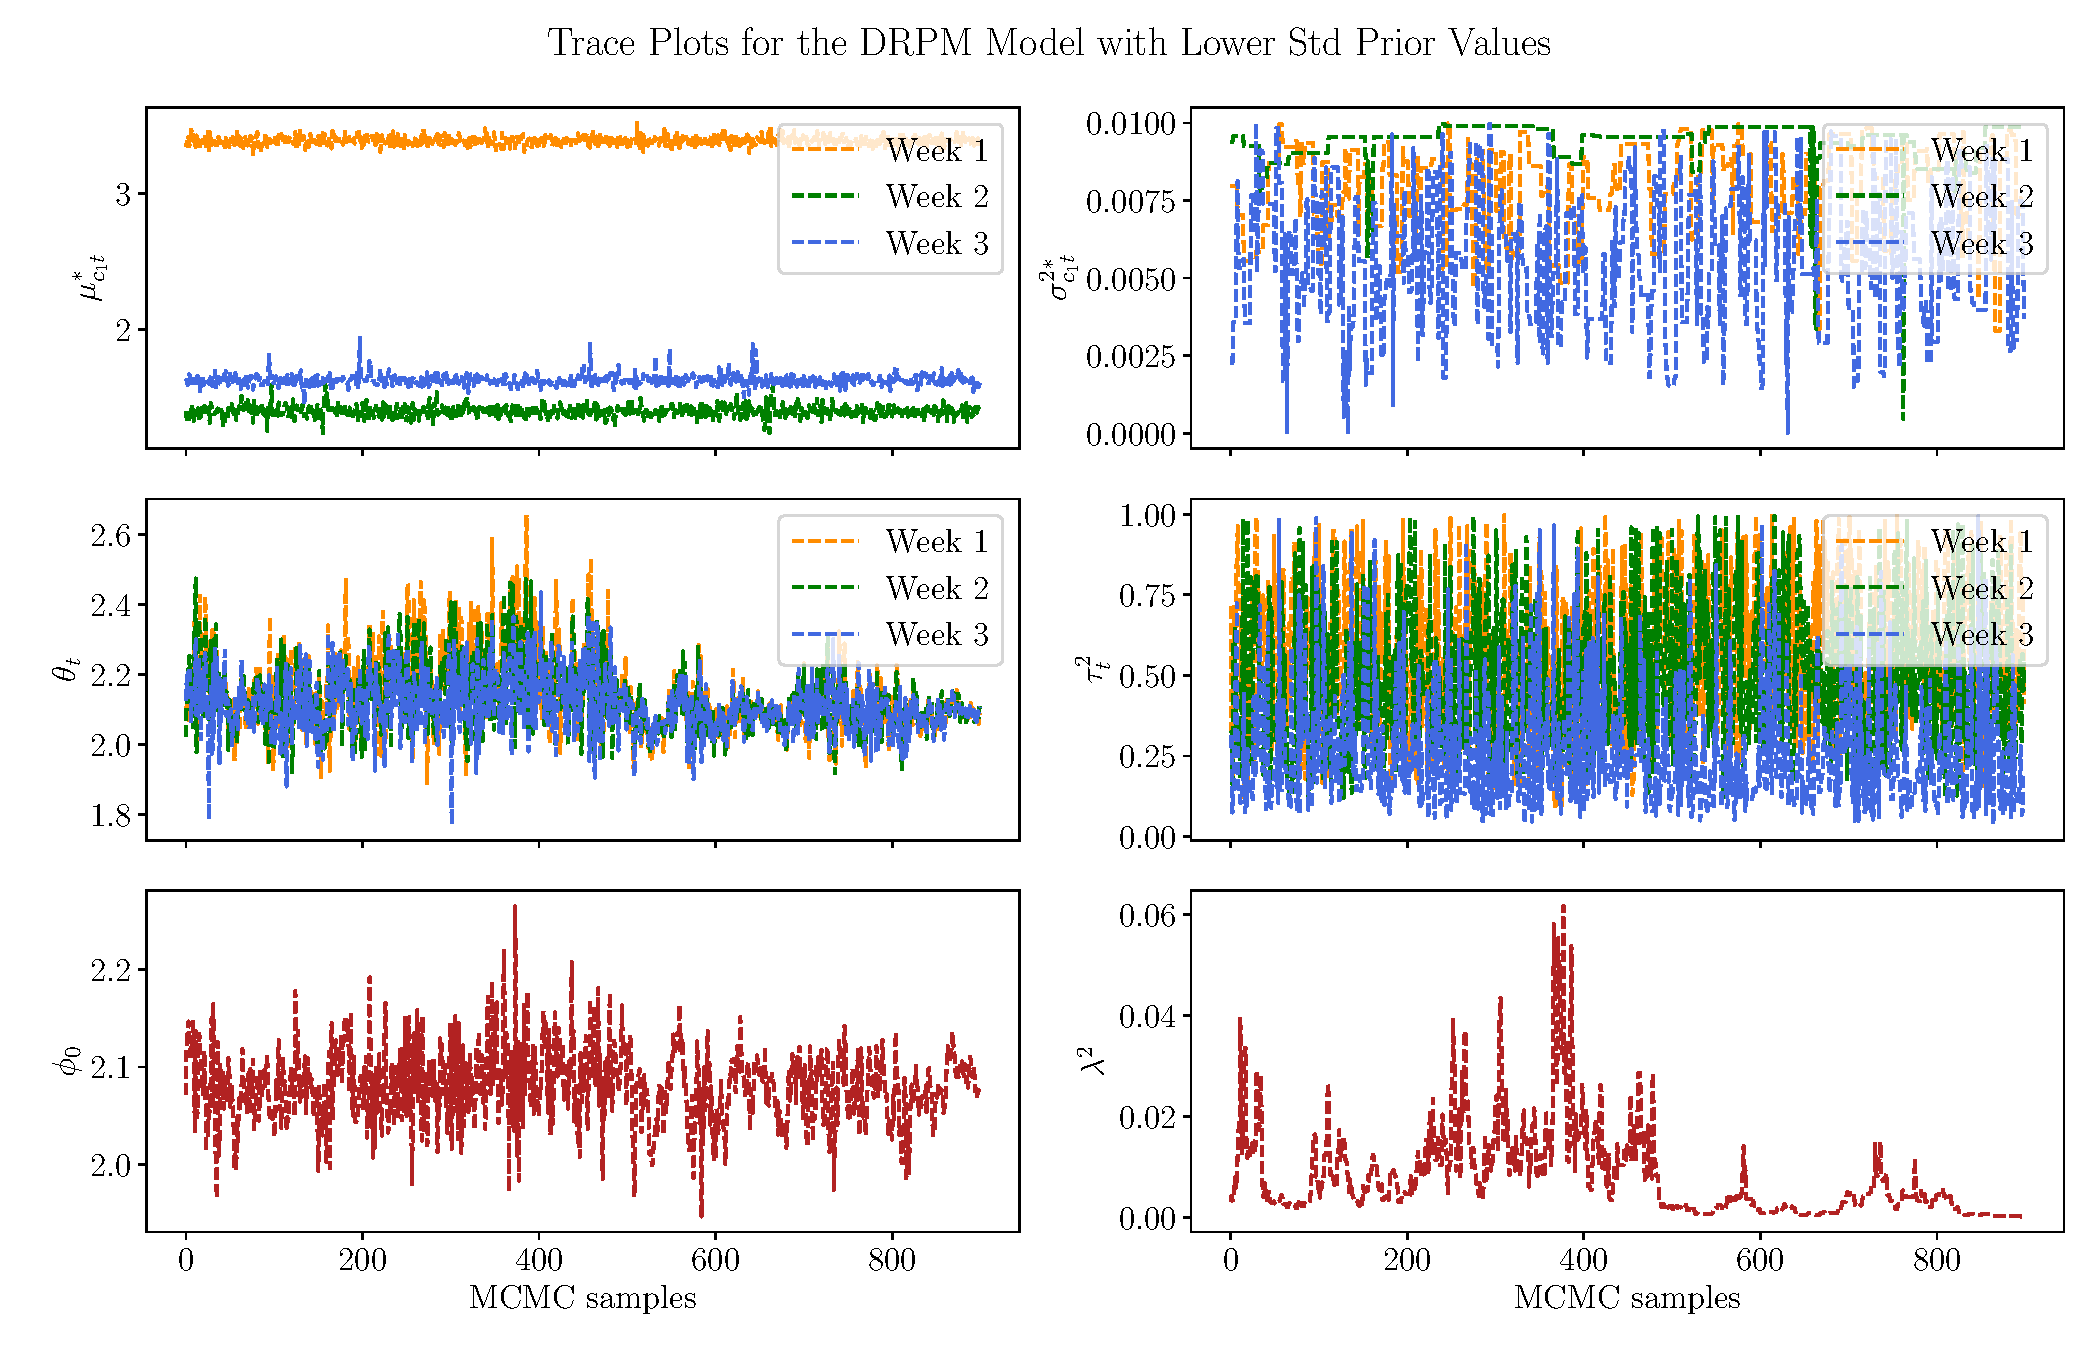
\includegraphics[width=.99\linewidth]{./imgs/drpm/drpm_lower_std_trace_plots.pdf}
    \caption{Trace Plots for the DRPM Model without spatial information parameters with the Lower Std Prior values. 
    Week-specific
    parameters are shown for the first three weeks of the year and cluster specific parameters are
    presented for the first cluster.}
    \label{fig:drpm_lower_std_trace_plots}
\end{figure}


\begin{figure}
     \centering
     \begin{subfigure}[b]{0.49\textwidth}
         \centering
         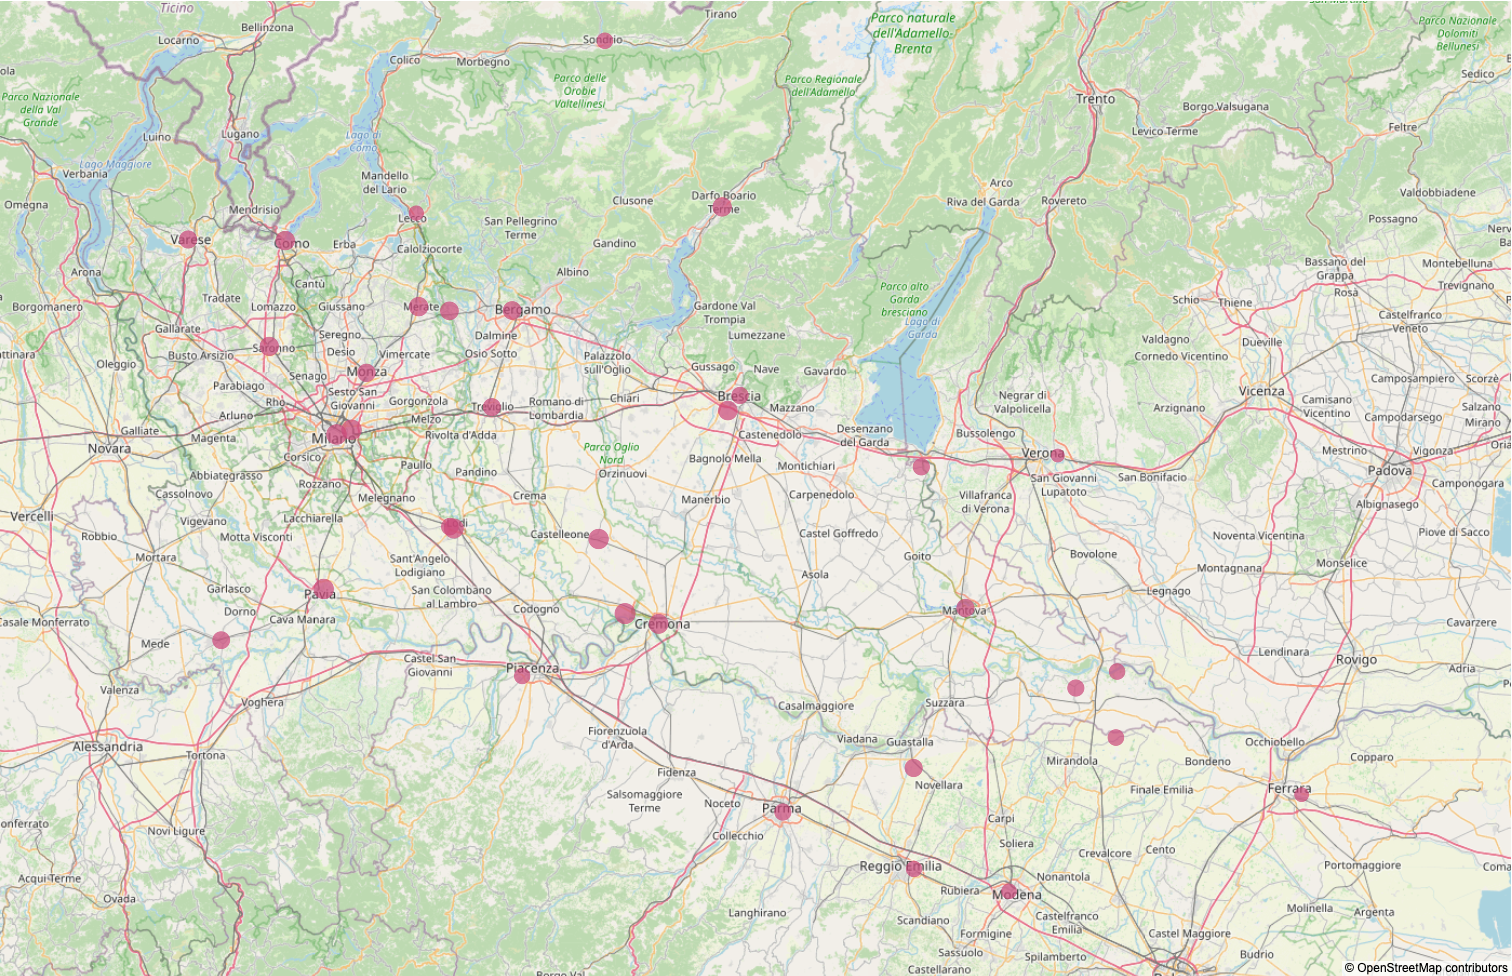
\includegraphics[width=\textwidth]{./imgs/drpm/drpm_base_clustering_paper_params.png}
         \caption{DRPM-Paper \cite{Page2021-Temporal}: 1 cluster in total.}
         \label{fig:DRPMclusteringPaper}
     \end{subfigure}
     \hfill
     \begin{subfigure}[b]{0.49\textwidth}
         \centering
         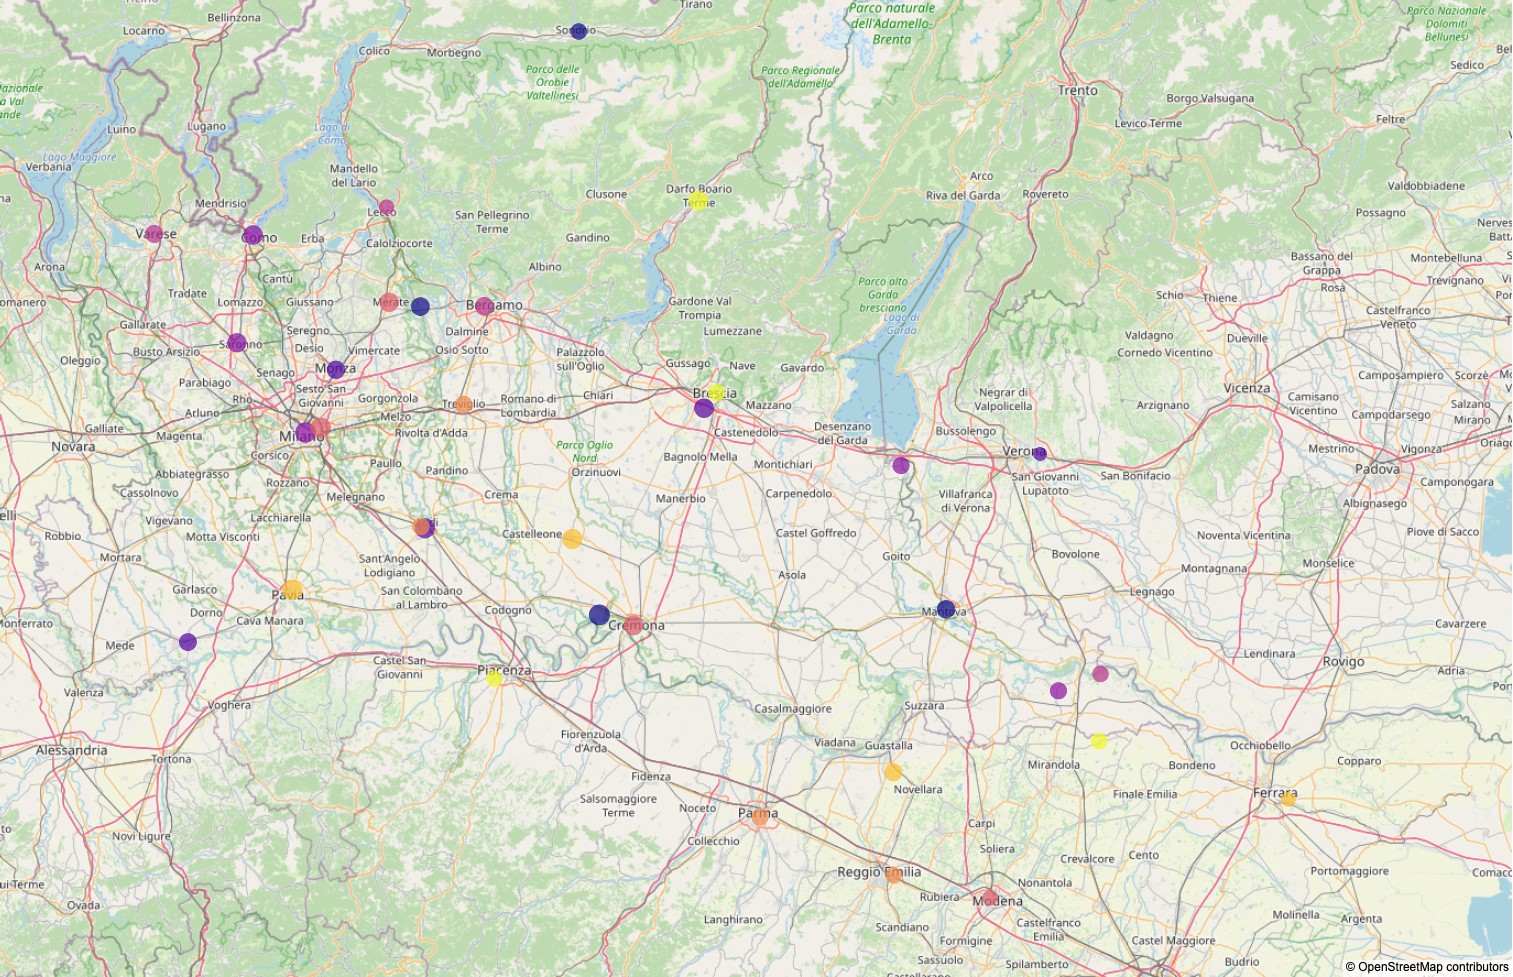
\includegraphics[width=\textwidth]{./imgs/drpm/drpm_base_clustering_lower_std.png}
         \caption{Lower Std (ours): 9 clusters in total.}
         \label{fig:DRPMClusteringLowerStd}
     \end{subfigure}
     \hfill
     \begin{subfigure}[b]{0.49\textwidth}
         \centering
         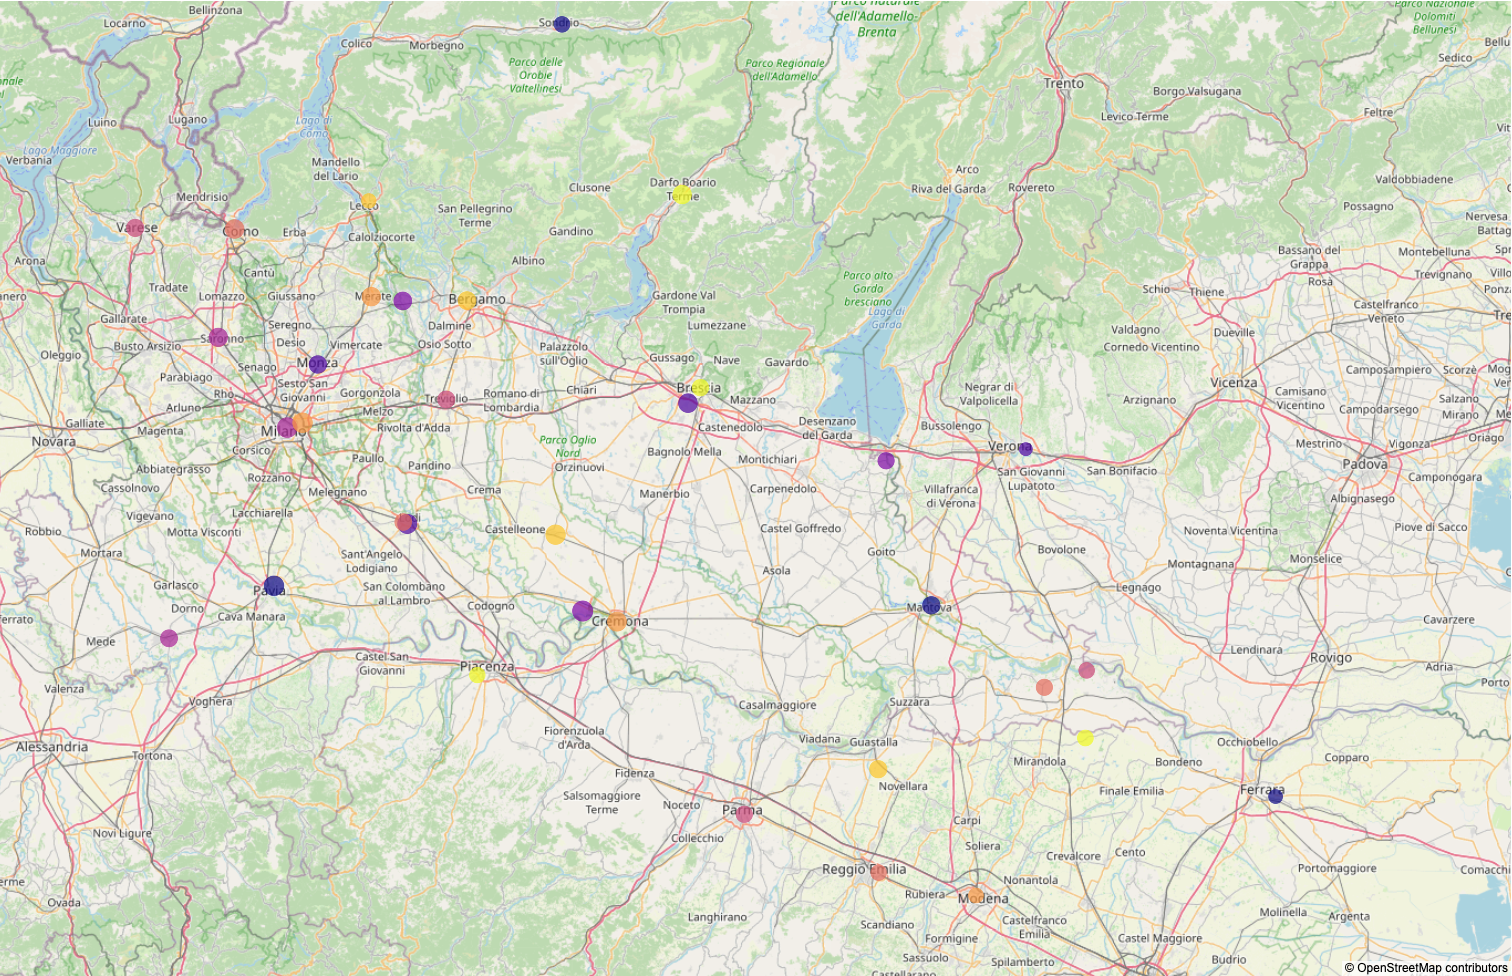
\includegraphics[width=\textwidth]{./imgs/drpm/drpm_base_clustering_mean_prev_year.png}
         \caption{Mean 2018 (ours): 13 clusters in total.}
         \label{fig:DRPMMeanPreviousYear}
     \end{subfigure}
        \caption{Exemplary clustering for week three of the year 2019 using all three of
        our base models without spatial information. All use the concentration parameter
        $M=0.1$ and the prior parameters listed in \cref{tab:DRPMPriorParam}. The color of
        the bubble indicates the cluster and the size of the bubble the weekly-average PM2.5 value.}
        \label{fig:DRPMClusteringBaseModels}
\end{figure}

\subsubsection{Spatially informed: Hyperparameter Gridsearch}
\subsubsection{Spatially informed: Extensions}
We fix a value of $M= 0.1$ and $\alpha_0 = 0.25$ for all of the experiments in this section, since our previous results emphasized
these two values as a good trade-off for all methods. Furthermore, the MSE is computed for all values in the log-space and is the
yearly-maximum MSE computed over all weekly MSEs. Given our
extension described in \cref{subsec:DRPMExtensions}, we compare our three base models by using a spatial-informed version of
DRPM and contrasting all possible combinations of temporal-dependency extensions.

In our notation $\eta_{10} =$ True indicates an AR(1)-type temporal-dependency in the likelihood,
$\phi_1 =$ True a temporal-dependency within the stations and $\alpha_t = $ True a temporal-dependency within
the partitions, i.e. $\alpha_t = $ False implies a constant value of $\alpha_t = \alpha_1$ over the entire time horizon
$t = 1, \ldots, T$. Finally, $g_i$ is the type of cohesion function used by the algorithm.

The results for our baseline version using the DRPM-Paper prior values is shown in \cref{tab:DRPMExtensionDRPMPaper} and
for the Lower Std and Mean 2018 version in \cref{tab:DRPMExtensionLowerStd} and \cref{tab:DRPMExtensionMean2018} respectively.

TODO: Evalation of the experiments and maybe another plot?

\begin{table}
\caption{\textbf{Spatially informed} DRPM Model for different hyperparameter configurations with the following prior values: $m_0 = 0.0$, $s_0^2 = 10000.0$, $A_\sigma = 10.0$, $A_\tau = 5.0$, $A_\lambda = 5.0$, $b = 1.0$, $a_\alpha = 2.0$, $b_\alpha = 2.0$ (\textbf{DRPM-Paper}).}
\centering\begin{tabular}{cccccccc}
\toprule
$\eta_{10}$ & $\phi_1$ & $\alpha_t$ & $g_i$ & LMPL & WAIC & Time [s] & MSE \\
\midrule
False & False & True & 3 & $-1.202 \cdot 10^{+03}$ & $2.382 \cdot 10^{+03}$ & $2.719 \cdot 10^{+01}$ & $1.248 \cdot 10^{+00}$ \\
False & False & True & 4 & $-1.217 \cdot 10^{+03}$ & $2.407 \cdot 10^{+03}$ & $2.854 \cdot 10^{+01}$ & $1.238 \cdot 10^{+00}$  \\
False & True & True & 3 & $-1.199 \cdot 10^{+03}$ & $2.378 \cdot 10^{+03}$ & $2.698 \cdot 10^{+01}$ & $1.256 \cdot 10^{+00}$  \\
False & True & True & 4 & $-1.226 \cdot 10^{+03}$ & $2.421 \cdot 10^{+03}$ & $3.068 \cdot 10^{+01}$ & $\mathbf{1.197 \cdot 10^{+00}}$  \\
True & False & True & 3 & $-1.329 \cdot 10^{+03}$ & $2.644 \cdot 10^{+03}$ & $2.726 \cdot 10^{+01}$ & $1.279 \cdot 10^{+00}$  \\
True & False & True & 4 & $-1.256 \cdot 10^{+03}$ & $2.486 \cdot 10^{+03}$ & $3.311 \cdot 10^{+01}$ & $1.235 \cdot 10^{+00}$  \\
True & True & True & 3 & $-1.710 \cdot 10^{+03}$ & $3.407 \cdot 10^{+03}$ & $2.721 \cdot 10^{+01}$ & $1.376 \cdot 10^{+00}$ \\
True & True & True & 4 & $-1.766 \cdot 10^{+03}$ & $3.500 \cdot 10^{+03}$ & $3.397 \cdot 10^{+01}$ & $1.391 \cdot 10^{+00}$ \\
False & False & False & 3 & $\mathbf{-1.198 \cdot 10^{+03}}$ & $\mathbf{2.375 \cdot 10^{+03}}$ & $\mathbf{2.647 \cdot 10^{+01}}$ & $1.221 \cdot 10^{+00}$  \\
False & False & False & 4 & $-1.275 \cdot 10^{+03}$ & $2.491 \cdot 10^{+03}$ & $4.507 \cdot 10^{+01}$ & $1.200 \cdot 10^{+00}$  \\
False & True & False & 3 & $-1.199 \cdot 10^{+03}$ & $2.376 \cdot 10^{+03}$ & $2.757 \cdot 10^{+01}$ & $1.237 \cdot 10^{+00}$ \\
False & True & False & 4 & $-1.264 \cdot 10^{+03}$ & $2.473 \cdot 10^{+03}$ & $4.155 \cdot 10^{+01}$ & $1.215 \cdot 10^{+00}$ \\
True & False & False & 3 & $-1.279 \cdot 10^{+03}$ & $2.545 \cdot 10^{+03}$ & $2.700 \cdot 10^{+01}$ & $1.262 \cdot 10^{+00}$ \\
True & False & False & 4 & $-1.958 \cdot 10^{+03}$ & $3.878 \cdot 10^{+03}$ & $4.503 \cdot 10^{+01}$ & $1.488 \cdot 10^{+00}$ \\
True & True & False & 3 & $-1.601 \cdot 10^{+03}$ & $3.189 \cdot 10^{+03}$ & $2.686 \cdot 10^{+01}$ & $1.343 \cdot 10^{+00}$ \\
True & True & False & 4 & $-1.937 \cdot 10^{+03}$ & $3.837 \cdot 10^{+03}$ & $4.398 \cdot 10^{+01}$ & $1.430 \cdot 10^{+00}$ \\
\bottomrule
\end{tabular}
\label{tab:DRPMExtensionDRPMPaper}
\end{table}

\begin{table}
\caption{\textbf{Spatially informed} DRPM Model for different hyperparameter configurations with the following prior values: $m_0 = 0.0$, $s_0^2 
= 200.0$, $A_\sigma = 0.1$, $A_\tau = 1.0$, $A_\lambda = 1.0$, $b = 1.0$, $a_\alpha = 1.0$, $b_\alpha = 1.0$ (\textbf{Lower Std})
A dash indicates that the package was not able to calculate the corresponding value.}
\centering\begin{tabular}{cccccccc}
\toprule
$\eta_{10}$ & $\phi_1$ & $\alpha_t$ & $g_i$ & LMPL & WAIC & Time & MSE \\
\midrule
False & False & True & 3 & $-\infty$ & $-3.154 \cdot 10^{+02}$ & $1.289 \cdot 10^{+02}$ & $1.690 \cdot 10^{+00}$ \\
False & False & True & 4 & $-$ & $-1.931 \cdot 10^{+02}$ & $2.315 \cdot 10^{+02}$ & $1.698 \cdot 10^{+00}$ \\
False & True & True & 3 & $-$ & $-3.572 \cdot 10^{+02}$ & $1.455 \cdot 10^{+02}$ & $1.695 \cdot 10^{+00}$ \\
False & True & True & 4 & $-$ & $3.747 \cdot 10^{+03}$ & $2.449 \cdot 10^{+02}$ & $1.705 \cdot 10^{+00}$ \\
True & False & True & 3 & $-$ & $4.923 \cdot 10^{+02}$ & $1.789 \cdot 10^{+02}$ & $1.708 \cdot 10^{+00}$ \\
True & False & True & 4 & $-$ & $-4.251 \cdot 10^{+02}$ & $2.020 \cdot 10^{+02}$ & $1.697 \cdot 10^{+00}$ \\
True & True & True & 3 & $\mathbf{-1.627 \cdot 10^{+03}}$ & $-3.593 \cdot 10^{+02}$ & $\mathbf{1.086 \cdot 10^{+02}}$ & $\mathbf{1.682 \cdot 10^{+00}}$ \\
True & True & True & 4 & $-$ & $3.429 \cdot 10^{+03}$ & $3.682 \cdot 10^{+02}$ & $1.702 \cdot 10^{+00}$ \\
False & False & False & 3 & $-$ & $-3.490 \cdot 10^{+02}$ & $1.345 \cdot 10^{+02}$ & $1.682 \cdot 10^{+00}$ \\
False & False & False & 4 & $-$ & $9.056 \cdot 10^{+00}$ & $2.713 \cdot 10^{+02}$ & $1.710 \cdot 10^{+00}$ \\
False & True & False & 3 & $-$ & $-4.750 \cdot 10^{+02}$ & $2.016 \cdot 10^{+02}$ & $1.695 \cdot 10^{+00}$ \\
False & True & False & 4 & $-$ & $\mathbf{-6.328 \cdot 10^{+02}}$ & $2.183 \cdot 10^{+02}$ & $1.697 \cdot 10^{+00}$ \\
True & False & False & 3 & $-$ & $2.319 \cdot 10^{+02}$ & $1.721 \cdot 10^{+02}$ & $1.697 \cdot 10^{+00}$ \\
True & False & False & 4 & $-$ & $-3.644 \cdot 10^{+02}$ & $2.026 \cdot 10^{+02}$ & $1.695 \cdot 10^{+00}$ \\
True & True & False & 3 & $-$ & $1.314 \cdot 10^{+02}$ & $1.452 \cdot 10^{+02}$ & $1.693 \cdot 10^{+00}$ \\
True & True & False & 4 & $-$ & $-1.356 \cdot 10^{+02}$ & $2.083 \cdot 10^{+02}$ & $1.695 \cdot 10^{+00}$ \\
\bottomrule
\end{tabular}
\label{tab:DRPMExtensionLowerStd}
\end{table}


\begin{table}
\caption{\textbf{Spatially informed} DRPM Model for different hyperparameter configurations with the following prior values: $m_0 = 2.91$, $s_0^2 
= 200.0$, $A_\sigma = 0.1$, $A_\tau = 1.0$, $A_\lambda = 1.0$, $b = 1.0$, $a_\alpha = 1.0$, $b_\alpha = 1.0$ (\textbf{Mean 2018}).
A dash indicates that the package was not able to calculate the corresponding value.
}
\centering\begin{tabular}{cccccccc}
\toprule
$\eta_{10}$ & $\phi_1$ & $\alpha_t$ & $g_i$ & LMPL & WAIC & Time & MSE \\
\midrule
False & False & True & 3 & $-$ & $-6.109 \cdot 10^{+02}$ & $1.245 \cdot 10^{+02}$ & $1.690 \cdot 10^{+00}$ \\
False & False & True & 4 & $-$ & $-3.894 \cdot 10^{+02}$ & $2.151 \cdot 10^{+02}$ & $1.700 \cdot 10^{+00}$ \\
False & True & True & 3 & $-5.115 \cdot 10^{+03}$ & $-4.875 \cdot 10^{+02}$ & $1.412 \cdot 10^{+02}$ & $1.685 \cdot 10^{+00}$ \\
False & True & True & 4 & $-$ & $-2.315 \cdot 10^{+02}$ & $2.505 \cdot 10^{+02}$ & $1.702 \cdot 10^{+00}$ \\
True & False & True & 3 & $-$ & $4.319 \cdot 10^{+02}$ & $\mathbf{1.073 \cdot 10^{+02}}$ & $\mathbf{1.674 \cdot 10^{+00}}$ \\
True & False & True & 4 & $-$ & $-1.461 \cdot 10^{+02}$ & $2.288 \cdot 10^{+02}$ & $1.702 \cdot 10^{+00}$ \\
True & True & True & 3 & $-$ & $5.938 \cdot 10^{+01}$ & $1.098 \cdot 10^{+02}$ & $1.684 \cdot 10^{+00}$ \\
True & True & True & 4 & $-$ & $-3.021 \cdot 10^{+02}$ & $2.043 \cdot 10^{+02}$ & $1.699 \cdot 10^{+00}$ \\
False & False & False & 3 & $-$ & $\mathbf{-6.850 \cdot 10^{+02}}$ & $1.817 \cdot 10^{+02}$ & $1.690 \cdot 10^{+00}$ \\
False & False & False & 4 & $-$ & $-4.635 \cdot 10^{+02}$ & $2.898 \cdot 10^{+02}$ & $1.701 \cdot 10^{+00}$ \\
False & True & False & 3 & $-$ & $-5.577 \cdot 10^{+02}$ & $1.536 \cdot 10^{+02}$ & $1.688 \cdot 10^{+00}$ \\
False & True & False & 4 & $-$ & $-2.545 \cdot 10^{+02}$ & $2.438 \cdot 10^{+02}$ & $1.708 \cdot 10^{+00}$ \\
True & False & False & 3 & $\mathbf{-2.353 \cdot 10^{+03}}$ & $-2.660 \cdot 10^{+02}$ & $1.189 \cdot 10^{+02}$ \\
True & False & False & 4 & $-$ & $-5.078 \cdot 10^{+02}$ & $2.501 \cdot 10^{+02}$ & $1.701 \cdot 10^{+00}$ \\
True & True & False & 3 & $-$ & $1.608 \cdot 10^{+04}$ & $4.449 \cdot 10^{+02}$ & $1.715 \cdot 10^{+00}$ \\
True & True & False & 4 & $-$ & $3.923 \cdot 10^{+03}$ & $2.871 \cdot 10^{+02}$ & $1.716 \cdot 10^{+00}$ \\
\bottomrule
\end{tabular}
\label{tab:DRPMExtensionMean2018}
\end{table}



\newpage

\section{Conclusions}



\vspace{0.5cm}

\newpage

%-----------------------------------------------------------------------------
% BIBLIOGRAPHY
%-----------------------------------------------------------------------------
\nocite{*}
\newpage
\printbibliography

\newpage

\section{Acknowledgements}
% \newpage
% \appendix
% \section{DRPM Model Results}
\end{document}